% {{{
\documentclass[a4paper,10pt,norsk]{article}
\usepackage[utf8]{inputenc}
\usepackage[norsk]{babel}
\usepackage{graphicx, verbatim, amsmath, amsfonts, geometry, float, import, bm}
\usepackage{siunitx} % converts expression to SI units/notation , \num{10e-10}
% \usepackage[hidelinks]{hyperref}
\usepackage{xcolor}
\usepackage[colorlinks = True,
            linkcolor = black,
            urlcolor  = blue,
            citecolor = blue,
            anchorcolor = blue]{hyperref}
\usepackage{biblatex}

% Code higligthing
\usepackage{listings}
\usepackage{xcolor}
\definecolor{codegreen}{rgb}{0,0.6,0}
\definecolor{codegray}{rgb}{0.5,0.5,0.5}
\definecolor{codepurple}{rgb}{0.58,0,0.82}

\lstdefinestyle{mystyle}{
    commentstyle=\color{codegreen},
    keywordstyle=\color{magenta},
    stringstyle=\color{codepurple},
    basicstyle=\ttfamily\footnotesize,
    breakatwhitespace=false,         
    breaklines=true,                 
    captionpos=b,                    
    keepspaces=true,                 
    numbersep=5pt,                  
    showspaces=false,                
    showstringspaces=false,
    showtabs=false,                  
    tabsize=4
}
\lstset{style=mystyle}
\setlength{\parindent}{0mm}
\setlength{\parskip}{1.5mm}

% }}}

\title{FYS-STK4155 - Project 3}
\author{Jens Junker Pedersen}

\begin{document}
\maketitle
\tableofcontents

%%%%%%%%%%%%%%%%%%%%%%%%%%%%%%%%%%%%%%%%%%%%%%%%%%%%%%%%%%%%%%%%%%%%%%%%%%%%%%%%%%%%%%%%%%
\section{Introduction}

% Motivation for feature selection
Feature selection is an important step in the machine learning process because
it helps reduce the complexity of the model and helps improve its accuracy. By
selecting the most relevant features, the model can better focus on the
important data points and ignore the noise. This can increase the accuracy of
the model and help reduce overfitting. Additionally, feature selection helps
reduce the time and resources required to train the model, which can be
especially helpful when dealing with large datasets.
Selecting good features will make the model more interpretable by removing redundant
or irrelevant features. 

% Radiomics and identification of features  
Radiomics is a field of medical imaging that uses advanced
image processing algorithms to extract quantitative features from medical
images such as CT, MRI, and PET scans. These features are then used to develop
predictive models to better understand a patient's disease and to predict
outcomes. Radiomics can be used to better understand the biology of cancer, to
develop personalized treatments, and to monitor the effectiveness of
treatments.

% Radiomics problem 
There are some serious challenges that needs to be solved in order for
Radiomics to be clinically relevant.     
A Radiomics feature should reflect the underlying pathology and not vary due to
changes in scanner type or scanner specific parameters. Different scanner
types, reconstruction and image processing parameters affect feature values
differently. These parameters need to be controlled in order for the field to have any
clinical relevance. 


% There is currently a high priority in the field to identify methods for
% harmonization features values. 

% TODO: write harmonization
% Feature harmonization in radiomics refers to the process of standardizing the
% calculation and representation of radiomic features across different imaging
% studies or datasets. This is important because radiomic features can be
% affected by various factors such as imaging modality, acquisition parameters,
% and image processing techniques, which can lead to significant variability in
% the calculated features even within a single study.

% To address this variability, feature harmonization involves establishing
% standardized protocols for calculating and representing radiomic features that
% can be applied consistently across different studies or datasets. 

By harmonizing the calculation and representation of radiomic features, it is
possible to more accurately compare and analyze the features across different
studies or datasets, enabling more reliable and reproducible results in
radiomics research.

% TODO: feature selection
% TODO: report structure
% robust with respect to scanner type and scanner specific parameters. Also
% different harmonization techniques    

% Problem non robust feature

% Dataest
In this report we will explore a lymphoma image dataset acquired with a PET % XXX add model
scanner. A total of n = 16 malignant tumors was identified in the image data 
Each image is reconstructed with different reconstruction protocols (our class
labels). A total of 15 radiomics features is extracted from the tumours (Volume
of Interest) 
% Objective: discriminate between reconstruction
We will explore simple machine learning algorithms to explore if it's possible
to discriminate between the different reconstruction methods. 

If a clear pattern between reconstruction algorithms exists, it may be possible to
transform features values between different reconstruction methods. And
therefore control for the specific reconstruction methods. In such a way that
it may be possible to define absolute standards for the interpretation of a specific
feature value and it's significance in terms of pathology. We will not try to
harmonize the data, but rather explore if harmonization models it's worth
exploring.  

% In this project we will use simple supervised machine learning algorithms to
% identify  

% What we have done
In the first part of the report we will implement simple feature selection
techniques to identify features that are able to discriminate between the
different PET reconstruction methods. We will use random forest to identify the
features with best discriminative power. Then we will use person correlation to
identify highly correlated redundant features. In the last part we will
use feed forward feature selection in conjugation with Support Vector Machine
(SVM). We will then evaluate if our prior analysis is in agreement with the
results obtained with SVM. If our models and selected features is able to
accurately discriminate between the different classes. Then, it may be possible
find models that are able to map feature values between series, and define
absolute standards for the quantitative meaning of a feature value with respect
to pathology. 

% Report structure
% Method 
The first part of the method section (\ref{sec:method_dataset}) explains how the data is organized and
how to reproduce the data with python code. Subsection
\ref{sec:method_descion_tree} and \ref{sec:method_random_forest} contains the
necessary theory on how to implement a random forest. The last part of
subsection \ref{sec:method_random_forest} explains how to reproduce our results
obtained with random forest feature selection. And also comparison of our own
implementation vs the sci-kit learn python library. The code used to produce
our results with the Random Forest algorithm can be found in the Github repository,
\url{https://github.com/jensjpedersen/Projects_FYS-STK4155/tree/main/Project3} 

% TODO Method SVM 
In \autoref{sec:SVM}, first the theory of Support Vector Machines is layed out and explained
in \autoref{sec:SVM_theory}. Then a code example is added to show how the SVM optimization problem might be solved
and an explanation of how we will utilize the SVM is given in \autoref{sec:SVM_method}. 
The code used to produce our results with SVM can be found in the Github repository,
\url{https://github.com/fredrikjp/FYS-STK4155/tree/master/Project3}. 



% Results random forest
The first part of our Discussion we present our results and discussion from
feature selection with Random Forest and Correlation analysis.  
Then the results and discussion from our Support Vector Machine is presented for 
different series classifications. 

Finally we summarize and conclude the project in the Conclusion section.  
% Results SVM 




%%%%%%%%%%%%%%%%%%%%%%%%%%%%%%%%%%%%%%%%%%%%%%%%%%%%%%%%%%%%%%%%%%%%%%%%%%%%%%%%%%%%%%%%%%
\section{Methods}
\paragraph{Resources Hyperlinks} 
\begin{itemize}
    \item \href{https://www.kaggle.com/code/rafjaa/dealing-with-very-small-datasets}{Dealing with very small datasets | Gaggle}
    
\end{itemize}


%%%%%%%%%%%%%%%%%%%%%%%%%%%%%%%%%%%%%%%%%%%%%
\subsection{Dataset}


Our dataset and all the source code can be found in the following gihtub
repository. 

Our dataset contains 14 features extracted on XXX:n different lymphoma. Each
feature is extract from a PET Scanner XXX: type where different image
reconstruction techniques was applied. In our analysis we will study 3
different reconstruction methods, XXX: names. This will be our classification
targets. Thus, we are interested to see if it is possibly to identify features
that gives good class separation with respect to reconstruction method. This
will be a challenging since our data only contains 16 samples per
reconstruction. This will be an exercise in selecting good features applied to
simple ML models


%%%%%%%%%%%%%%%%%%%%%%%%%%%%%%%%%%%%%%%%%%%%%
\subsection{Random forest}
In our first attempt to identify good features (features with good
class separation), we will use a random forest classifier. 
It can be used to identify the features and feature value that splits the data
into the purest classes (see XXX)
The algorithm works by constructing multiple decision trees, each of which is trained 
on a subset of the data. 

\subsubsection{Decision Tree Classifier}
A classification decision tree is a predictive model that predicts the target
class of a feature based on a set of binary rules . The decision tree consists of a series of
nodes, branches, and leaves. Each node represents a decision point, each branch
represents a possible outcome, and each leaf represents a final consequence or
result. 

% XXX: explain fig
% and structure in a decision tree
\begin{figure}[H]
    \centering
    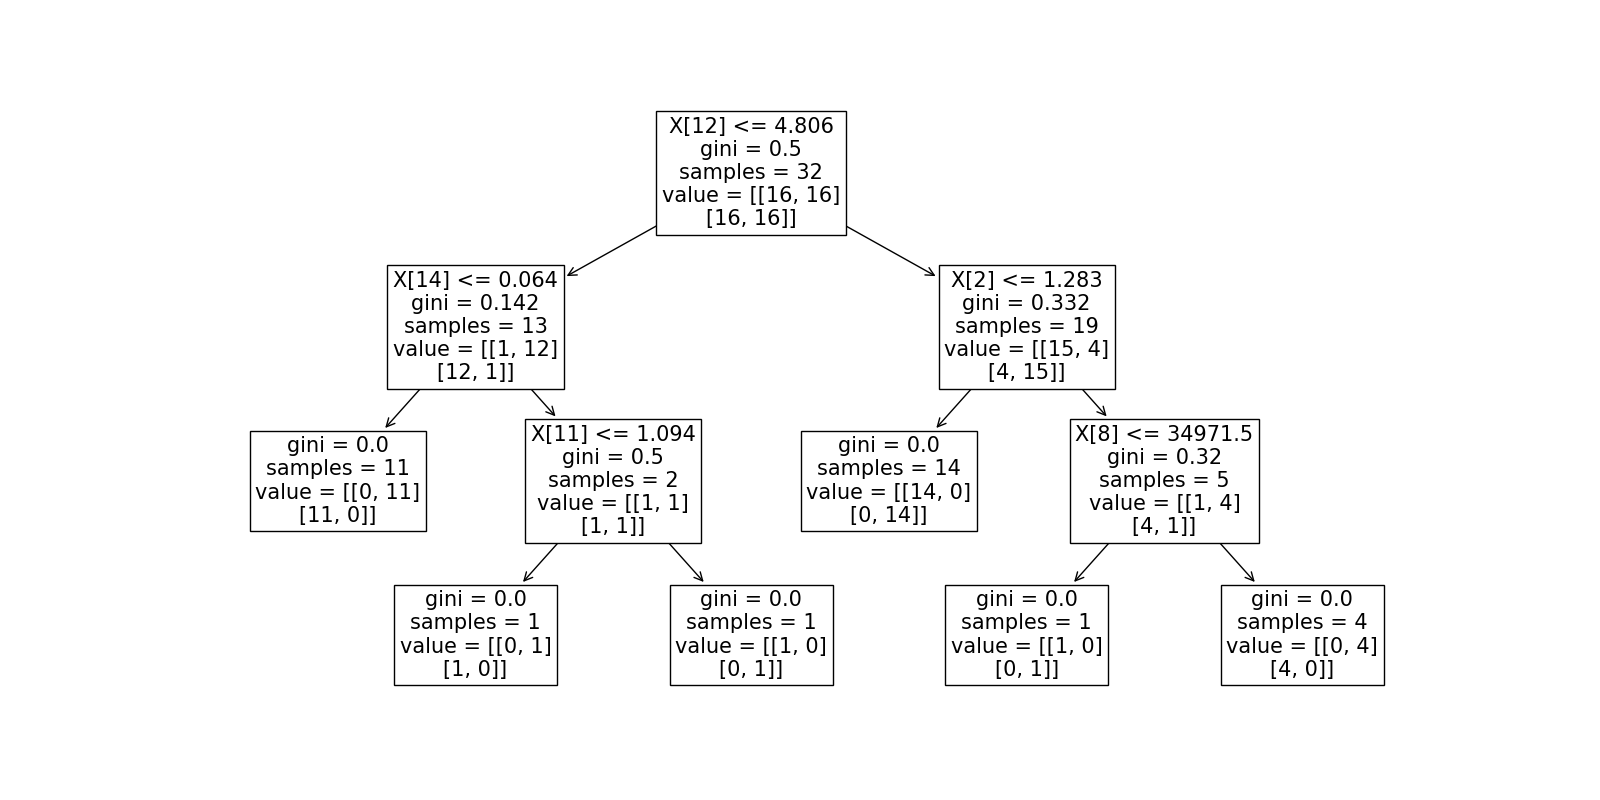
\includegraphics[width=0.8\textwidth]{Figures/descion_tree.png}
    \caption{Decision tree}  
    \label{fig:descision_tree} 
\end{figure}

A typical structure of a decision is shown in figure \ref{fig:descision_tree}. Each rectangle
represents a node in the tree. The build of a decision consists of finding
the feature and feature value (threshold) at each node that maximizes the
purity of each child node resulting from the split. At each node the data is
split into two child nodes based on the threshold value. Values lower than the threshold is
passed to the left child node and values higher is passed to the right child
node. Thus, the tree consists of a set of rules on where to a specific sample. The algorithm is recursive and starts at the
root node (the upper rectangle) on continues until a Leaf node is reached.
That is, one of the squares in the bottom of the figures.     


\paragraph{The CART algorithm} \hfill

We implemented the CART algorithm to find the optimal splits in the data.  

The CART algorithm splits the data set in two subsets using a single feature
$k$ and a threshold $t_k$ \cite{w44}. The purity of the split is then evaluated
with the cost function: 
\begin{equation*}
    \label{eq:cart} 
    C(k, t_k) = \frac{m_{\text{left}} }{m} G_{\text{left}}+
    \frac{m_{\text{right}} }{m} G_{\text{right}}, 
\end{equation*}

where $G$ is a measure of impurity (see section ),
$m_{\text{left}} $ and $m_{\text{right}} $ is the number of samples in the left
and right subsets resulting from the split. The total number of samples is $m =
m_{left} + m_{right}  $ 

The algorithm iterates through all p features and n samples. For each feature k
and threshod $t_k$, the cost score is evaluated on the two subsets. The
threshold and features that produced the best score is stored in a node. This
process is repeated on the data subsets in a recursive way until a specific
criterion is met. This produces a leaf node in the tree. 

In our implementation the recursion stops if it is not possible to split the
subset further. That is, the number of samples in the subset is equal to one.   
The recursion will also stop if our subset is 100\% pure. That is, the subset
only consist of one class label.  

\paragraph{Gini factor} \label{sec:gini_factor} \hfill

The Gini factor is used to measure the purity of the data subset and is
calculated as:
\begin{equation*}
    G = 1 - \sum_{i=1}^{c} P_i ^2 
\end{equation*}
where $P_i$ is the probability that a sample belongs to class i. 

For a maximum impurity, where $P_1 = P_2 = 0.5$ the Gini factor is 0.5. A
smaller value indicates a better split. For a perfectly pure class the Gini
factor is 1. That is all the samples belongs to a class k ($P_k = 1$).     


Our class target labels was stored in one hot vector of size $n \times c$, 
where n is the number of samples in the data subset and c is the number of
classes. The probability of each class was calculated with this python snippet:
\begin{lstlisting}[language=Python]
import numpy as np
P = np.sum(y, axis = 0)/y.shape[0]
\end{lstlisting},
where \verb|y| is the one hot vector of our class targets. 

\paragraph{Calculating the feature importance} \hfill
Our random forest implementation was used to identify most discriminative
features and not used for its predictive power. Again, we will use the Gini
factor to calculate the feature importance. 


We want to quantify the impurity decrease as results of a feature split.
Therefore, we are interested in the change in impurity with respect to a node and its
child nodes. The impurity decrease also needs to take into account the number
of samples. A feature is more important if it is able to separate more samples.       

% We will use the same formula as the scikit learn python library \cite{sklearn}
to estimate the feature importance: 
\begin{equation*}
    \frac{m}{M} \cdot (G  - \frac{m_{\text{left}} }{m} G_{\text{left}}+
    \frac{m_{\text{right}} }{m} G_{\text{right}}), 
\end{equation*}
where $G$, $G_{left} $ and $G_{right} $ as the Gini factor for the parent,
left child and right child node respectively. M is the total number of samples
in our input data. The other quantities are as defined in equation
\ref{eq:cart}. 

All our decision trees has a variable called \verb|feature_importances_|, which
contains the impurity decrease obtained from the best split of a node (except
for leaf nodes).   

When building the tree all features is considered each time a node is to be
split. If the same feature is used multiple times to split nodes in to a tree.
Then, only the split that produces the highest impurity decrease is stored in
the \verb|feature_importances_| variable. Hence, used to evaluate the feature
importance.      



Our decision tree algorithm can be used directly to identify good features.
However, there are some problems. The algorithm usually produces very different
results dependent on small variations in the data. That is, classification
decision trees suffers from high variance. It may also neglect highly
correlated features that produces a slightly poorer separation. To circumvent
these problems we implemented the random forest algorithm. 

%%%%%%%%%%%%%%%%%%%%%%%%%%%%%%%%%%%%%%%%%%%%%
\subsection{Random forest}
Random forest is a type of ensemble learning method, which uses multiple
decision trees to make predictions and combines them to create a more accurate
and stable prediction. It uses a technique called bagging, which involves
randomly selecting a subset of data from the training set and building a
decision tree from each subset. 

It also uses feature resampling to reduce the
overfitting of the model. We will implement feature resampling
to better evaluate the performance of all the features. Feature resampling is
done within each node of the descion tree. Hence, the best split at each node is
evaluated on different feature subsets. The general algorithm for a descion
tree is listed below. 
\paragraph{Algorithm} 

% Random forest algorithm - cite lecture 44
\fbox{\begin{minipage}{30em}
We will grow of forest of say $\bm{B}$ trees.

For b=1:B

Draw a bootstrap sample from the training data organized in our $\boldsymbol{X}$ matrix.

We grow then a random forest tree $T_b $
based on the bootstrapped data by repeating the steps outlined till we reach
the maximum node size is reached

we select $m \leq p$  variables at random from the p predictors/features

pick the best split point among the $m$ features using for the CART
algorithm and create a new node

split the node into daughter nodes

Output then the ensemble of trees $\{T_b\}^B_1$

and make predictions for either a regression type of problem or a
classification type of problem.


\end{minipage}}

















% What is one hot vector?
% A one hot vector is a vector of all zeros, except for a single element which is set to one. 
% It is commonly used to represent a categorical variable in machine learning models.


1. Start by selecting the best attribute from the dataset. This attribute will be the root node of the decision 
tree. 

2. Split the data into subsets based on the attribute selected in the first step. 

3. For each subset, select the best attribute and create a decision tree node.

4. Repeat the process for each subset until all the data points have been classified.

5. Finally, test the accuracy of the decision tree by running it on a different set of data.
















\paragraph{Overview} 
\begin{enumerate}
    \item Identify good features by visual inspection 
    \item Feature reduction:
        \begin{itemize}
            \item Manual:
                \begin{itemize}
                    \item Remove correlated features
                \end{itemize}
                
            \item Automatic:
                \begin{itemize}
                    \item Iterate all the features and find best model 
                \end{itemize}
                
        \end{itemize}
        
    \item Evaluate results and find the best ML classification algorithm for dataset 
    
\end{enumerate}


%%%%%%%%%%%%%%%%%%%%%%%%%%%%%%%%%%%%%%%%%%%%%
\subsection{Feature section}
\begin{itemize}
    \item not correlated
    \item highly dependent on target variable 
\end{itemize}




%%%%%%%%%%%%%%%%%%%%%%%%%%%%%%%%%%%%%%%%%%%%%
\subsection{Dataset and model selection}
\begin{itemize}
    \item Bagging - Bootstrap aggregation
    \item Random forest
\end{itemize}

\begin{itemize}
    \item Sparse data $ \rightarrow $ Focus on simple ML methods
    \item ML classification algorithms suited for sparse data: 
        \begin{itemize}
            \item SVM
        \end{itemize}
        
\end{itemize}



\paragraph{ANOVA} 
Used to select features that is highly dependent on the target variable
\cite{anova}. 











\subsubsection{SVM}
Support Vector Machine (SVM) is a machine learning method used for 
classification and regression problems. We will use SVM for binary 
classification where the algorithm's aim is to create a $p-1$ dimensional
affine subspace of the $p$ dimensional feature space which distinguishes all the 
classifications optimally. This subspace is called a hyperplane and the 
optimal hyperplane maximizes the margin which is the distance from the 
hyperplane to the nearest data point in feature space. The optimal hyperplane 
will therefore be the same distance from the nearest point(s) of each 
classification it divides. These points are called the support vectors.

The hyperplane is defined by a $p$ dimensional weight vector $\boldsymbol{w}$ and a 
bias term $b$
\begin{equation}
\boldsymbol{x^T}\boldsymbol{w} + b =0, 
\label{eq:hyperplane}
\end{equation}
where $\boldsymbol{x^T}=[x_1,x_2,...,x_p]$ is the transpose of a point in feature space.
Separating our classifications by $y_i=1$ or $y_i=-1$, we can classify a 
data point $x_i$ with our hyperplane as 
\begin{gather*}
y_i = sign(\boldsymbol{w^T}\boldsymbol{x_i}+b). 
\end{gather*}
Our margin defined by our hyperplane and training points $x_i$ with classification $y_i$ becomes the largest $M$ such that 
\begin{gather}
\frac{1}{||\boldsymbol{w}||}y_i(\boldsymbol{w^Tx_i}+b) \ge M, \forall i=1,2,...,p. 
\end{gather}
If we scale this equation such that $||\boldsymbol{w}||=1/M$, finding the maximal margin 
will be equivalent to minimizing 
\begin{gather*}
||\boldsymbol{w}||
\end{gather*}
subject to the constraints 
\begin{gather*}
y_i(\boldsymbol{w^Tx_i}+b) \ge 1, \forall i.
\end{gather*}

The optimization of the hyperplane can be solved using Lagrange multipliers. 
For each constraint formulated as $\phi_k (\boldsymbol{x})=0$, we add a Lagrange
multiplier $\lambda _k \ge 0$ such that $\frac{\partial f}{\partial x_i}+\lambda_k \frac{\partial \phi }{\partial x_i}=0$,
where $f(\boldsymbol{x})$ with $x_i \epsilon [\boldsymbol{x}]$ is the function we want to minimize 
subject to the constraints.

Using the Lagrange multipliers, the optimization problem can be solved by minimizing 
the following Lagrangian function
\begin{equation}
	L(\lambda ,b,\boldsymbol{w})=\frac{1}{2}\boldsymbol{w^Tw}-\sum_{i} \lambda _i[y_i(\boldsymbol{w^Tx_i}+b)]-1,\lambda _i \ge0. 
	\label{eq:Lagrangian}
\end{equation}
Taking the derivatives with respect to $\boldsymbol{w}$ and $b$ we obtain the constraints 
\begin{gather*}
\frac{\partial L}{\partial b}=-\sum_{i} \lambda _i y_i=0,
\quad \frac{\partial L}{\partial \boldsymbol{w} }= \boldsymbol{w} -\sum_{i} \lambda _i y_i \boldsymbol{x_i} =0.
\end{gather*}
Inserting these constraints in \autoref{eq:Lagrangian}, we are able to get rid 
of the variables $\boldsymbol{w}$ and $b$ from the Lagrangian
\begin{equation}
L = \sum_{i} \lambda _i - \frac{1}{2}\sum_{ij}^{n} \lambda _i \lambda _j y_i y_j \boldsymbol{x_i^Tx_j},
\label{eq:Lagrangian_lmb}
\end{equation}
with constraints $\lambda _i \ge 0$ and $\sum_{i} \lambda _iy_i=0$.
Additionally, the Karush-Kuhn-Tucker condition has to be satisfied
\begin{gather*}
\lambda _i >0 \implies y_i(\boldsymbol{w^Tx_i}+b)=1, \quad y_i(\boldsymbol{w^Tx_i}+b)>1 \implies \lambda _i = 0,
\end{gather*}
such that $\lambda _i>0$ if and only if $\boldsymbol{x_i}$ is a support vector. 

There is often overlap between classifications in feature space. Then, there 
won't exist a hyperplane able to separate all the classifications. We will 
implement two ways to deal with this problem. 

The first is to introduce slack variables. The slack variables 
$\varepsilon _i \ge  0$ allows for some misclassification of 
the training data. The amount of misclassification is governed by the 
slack constant $C$ which sets a bound on the sum of the slack variables.  
Utilizing this method turns our SVM in to a so-called soft classifier as 
opposed to a hard classifier. 
The Lagrangian stays the same as \autoref{eq:Lagrangian_lmb}, but 
with different constraints:
\begin{gather*}
	\sum_{i} \lambda _i y_i = 0, \quad 0 \le \gamma _i \le C,\\
	\lambda _i[y_i(\boldsymbol{w^Tx_i}+b)-(1-\varepsilon _i)]=0,\\
y_i(\boldsymbol{w^Tx_i}+b)-(1-\varepsilon _i) \ge 0.
\end{gather*}

The second method is to transform the basis of the feature space to obtain 
better separation between classifications. This is done with a so-called 
kernel $K$ which transforms the data in \autoref{eq:Lagrangian_lmb} by 
\begin{gather*}
\boldsymbol{x_i^Tx_j} \rightarrow ø(\boldsymbol{x_i})^Tø(\boldsymbol{x_j})=K(\boldsymbol{x_i,x_j}),
\end{gather*}
where $ø(\boldsymbol{x})$ is some transformation of the feature space.

Our Lagrangian in \autoref{eq:Lagrangian_lmb} expressed as a convex optimization 
problem in terms of a matrix equation using a kernel $K$ may be written as 
\begin{equation}
\frac{1}{2}\boldsymbol{\lambda ^T}
\begin{bmatrix}
	 y_1y_1K(\boldsymbol{x_1,x_1})  & y_1y_2K(\boldsymbol{x_1,x_2}) & \hdots & y_1y_nK(\boldsymbol{x_1,x_n}) \\
	 y_2y_1K(\boldsymbol{x_2,x_1})  & y_2y_2K(\boldsymbol{x_2,x_2}) & \hdots & y_2y_nK(\boldsymbol{x_2,x_n}) \\
	\vdots & \vdots & \ddots & \vdots \\
	 y_ny_1K(\boldsymbol{x_n,x_1})  & y_ny_2K(\boldsymbol{x_n,x_2}) & \hdots & y_ny_nK(\boldsymbol{x_n,x_n}) \\
\end{bmatrix}
\boldsymbol{\lambda }-\mathbb{1}\boldsymbol{\lambda },
\label{eq:Lagrangian_mateq}
\end{equation}
where $\mathbb{1}=[1,1,...,1]$ is $n$ dimensional. Here $\boldsymbol{\lambda }=[\lambda _1,\lambda _2,...,\lambda _n]^T$ 
and $\boldsymbol{y}=[y_1,y_2,...,y_n]^T$. The constraints can be written as 
$\boldsymbol{y^T\lambda }=0$, and $0 \le \lambda _i \le C$ assuming we are using 
a slack constant $C$.  

There are many popular kernels such as the Gaussian radial basis function which 
we will use:
\begin{equation}
K(\boldsymbol{x_i,x_j})=exp(-\gamma ||\boldsymbol{x_i-x_j}||^2).
\label{eq:grbf}
\end{equation}
Here, $\gamma $ is a constant which needs to be tuned.
We know that the feature space transformation $ø$ defining the kernel exists based 
on Mercer's theorem which states that if $K$ is symmetric, continuous and leads to 
a positive semi-definite matrix $P$ defined in \autoref{eq:Lagrangian_mateq}, then 
$ø$ exists. 

To minimize \autoref{eq:Lagrangian_mateq}, we will use \verb|solvers.qp| from
the python library \verb|cvxopt|. The solver takes the minimization problem 
and its constraints as matrix equations:
\begin{equation}
	\begin{split}
		\text{min}_{\boldsymbol{\lambda }}\quad \frac{1}{2}\boldsymbol{\lambda ^TP\lambda +q^T\lambda },\\
	\text{subject to}\quad \boldsymbol{G \lambda  \le h}, \quad \boldsymbol{A \lambda =b}.
	\end{split}
	\label{eq:solver_eq}
\end{equation}

The problem in \autoref{eq:solver_eq} are defined and solved based on \autoref{eq:Lagrangian_mateq}
in the following code:
\begin{lstlisting}[language=Python]
def solve(self):
        # Solution for minimizing 
        # (1/2) * lambda.T @ P @ lambda + q.T @ lambda 
        # subject to constraints

        y = self.y_train
        X = self.X_train
        n = self.X_train.shape[0]

        q = -1 * np.ones(n).T
        P = np.zeros((n, n))
        for i in range(n):
            for j in range(n):
                P[i,j] = y[i] * y[j] * self.K(X[i,:], X[j,:])
        
        # G and h sets constraints on col vec lambda: G@lambda <= h
        G = np.zeros((2*n, n))
        G [:n, :] = np.identity(n) * (- 1)
        G[n:,:] = np.identity(n)
        h = np.zeros(2*n)
        h[n:] = np.ones(n) * self.C
        # A and b sets  constraints on labda: A@lambda = b
        A = np.array(self.y_train, dtype=float).T
        b = np.zeros(1) 
    
        # Solve 
        P, q, G, h, A, b = matrix(P), matrix(q), matrix(G), matrix(h), matrix(A), matrix(b)
        solvers.options['show_progress'] = False
        sol = solvers.qp(P, q, G, h, A, b)
        self.lmb = np.array(sol["x"])
        self.lmb_non_zero_indecies = np.where(self.lmb > 1e-5)[0]
        self.calc_b()
\end{lstlisting}



%%%%%%%%%%%%%%%%%%%%%%%%%%%%%%%%%%%%%%%%%%%%%%%%%%%%%%%%%%%%%%%%%%%%%%%%%%%%%%%%%%%%%%%%%%
\section{Discussion}

%%%%%%%%%%%%%%%%%%%%%%%%%%%%%%%%%%%%%%%%%%%%%
\subsection{Manual feature selection}

% sklearn random forest  

\begin{table}[H]
    \centering
    \caption{Ranking of feature importance from best to worst with respect to
    impurity decrease for three different reconstruction methods on the full
    dataset obtained with sci-kit learn.}  
    \label{tab:feature_importance}  

    \begin{tabular}{|c|c|c|c|}
        \hline
        Rank & Feature index & Feature name & Impurity decrease \\     
        \hline
        0       & 2           & histogram min  & 0.102915  \\
        1      & 12            & glcm entropy  & 0.088981  \\
        2      & 11           & glcm contrast  & 0.083777  \\
        3       & 4           & histogram std  & 0.081181  \\
        4      & 13        & glcm homogeneity  & 0.080463  \\
        5       & 5      & shape area\_density  & 0.073690  \\
        6       & 3          & histogram peak  & 0.069483  \\
        7       & 0           & histogram max  & 0.064857  \\
        8      & 14      & glcm joint\_maximum  & 0.061548  \\
        9       & 9    & shape volume\_density  & 0.055089  \\
        10      & 8            & shape volume  & 0.051088  \\
        11      & 7           & shape surface  & 0.048897  \\
        12     & 10            & glcm cluster  & 0.048494  \\
        13      & 1          & histogram mean  & 0.047758  \\
        14      & 6  & shape convex\_hull\_area  & 0.041778  \\
        \hline
         
    \end{tabular} 
\end{table}


% Identify features with poor class separation

% Identify highly correlated features  
% * plot correlation matrix  

\begin{figure}[H]
    \centering
    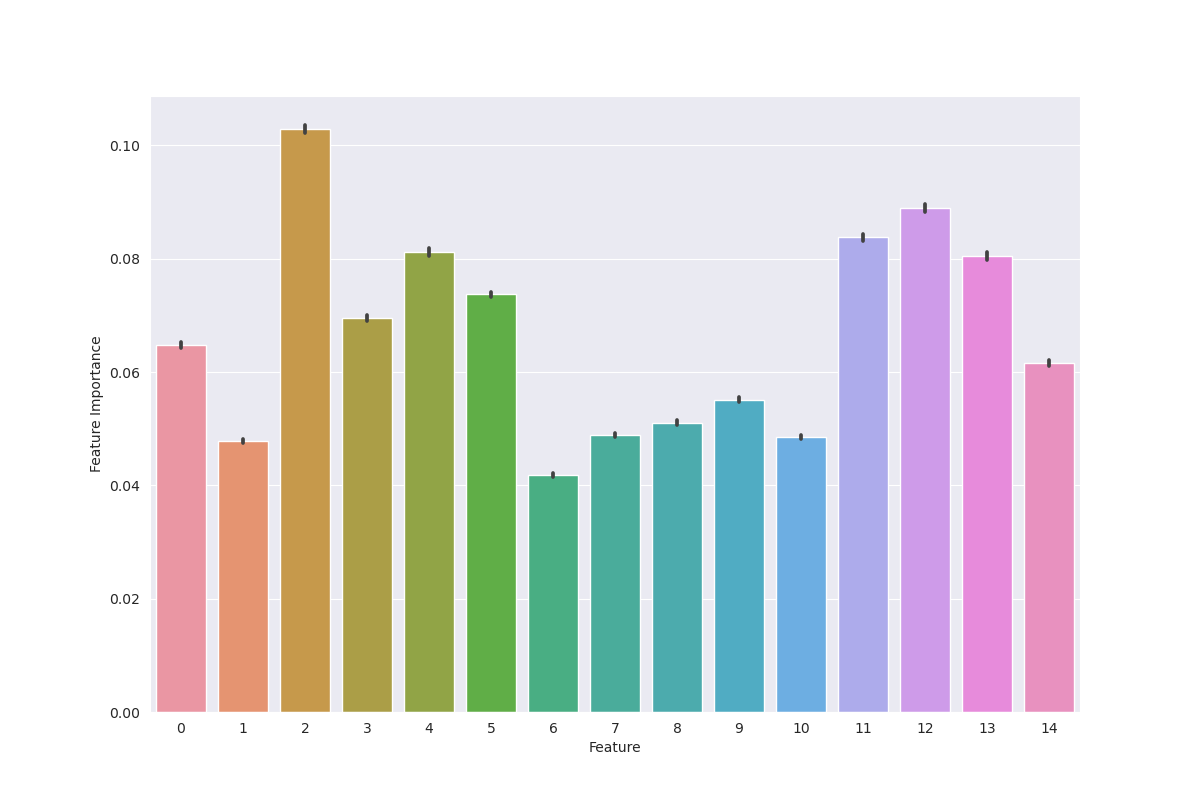
\includegraphics[width=0.8\textwidth]{Figures/feature_importance_sklearn_3s.png}
    \caption{Mean of the feautre\_importacnes\_ (purity decrease) for each decision tree. The
    error bar shows the 95\% confidence interval. The x-axis represent feature
    number as defined in table \ref{tab:feature_names}.  }  
    \label{fig:feature_importance} 
\end{figure}

% \begin{figure}[H]
%     \centering
%     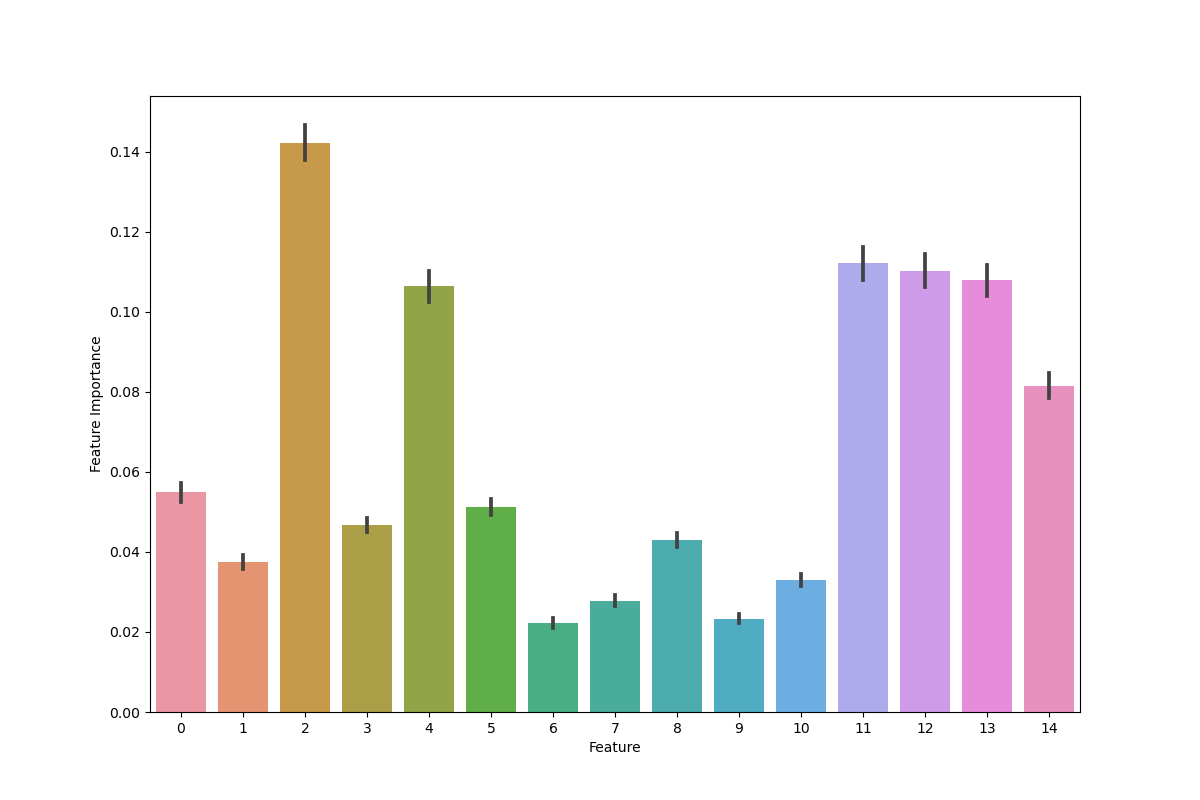
\includegraphics[width=0.8\textwidth]{Figures/feature_importance.png}
%     \caption{Mean of the feautre\_importacnes\_ (purity decrease) for each decision tree. The
%     error bar shows the 95\% confidence interval. The x-axis represent feature
%     number as defined in table XXX: ref table.  }  
%     \label{fig:feature_importance} 
% \end{figure}

Figure \ref{fig:feature_importance} shows the histogram the feature importance
on the y axis and feature index on the x axis. These results was obtained with
with sci-kit learn's implementation of the random forest. The 95 \% confidence
interval is shown on the top of each bar. The histogram min is best able to
discriminate between the tree different reconstruction methods, with a impurity
decrease of 0.1029\&. The numerical feature importance (Impurity decrease)
values for all the features is listed in table \ref{tab:feature_importance}.
The glcm entropy features gives the second best impurity decrease with a value
of 0.0890. Our next 3 best features are glcm contrast, histogram std and glcm
homogeneity which performs similarity with an impurity descrese in the rande
0.0805-0.0838. 

In figure \ref{fig:correlation} the correlation between all the features is
plotted. The color bar has a range from -1 (black) to 1 (white), where a score
of 1 indicates perfect correlation. The histogram min features is not strongly
correlated with any other features, thus we expect this features give a good
accuracy on the test data with the SVM model. Our next best features glcm
entorpy is highly correlated with histogram std. Thus, only one of the features
should be used when training a classification model. Utilizing both features
will produce high variance due to redundant information. When training our SVM
we therefore expect the combinations of these two features to produce worse
accuracy on the test data compared with any other combination of the top 5
features. Glcm contrast has the highest correlation with histogram std, but not
to the same extent as the two previous discussed features. GLCM homogeneity has
the highest correlation with glcm joint\_maximum. However, the GLCM maximum
features performance significantly worse with a difference impurity decrease of
0.0189. In our training of the SVM we expect that a combination of hisogram
min, glcm entropy. The 4 combinations of features we expect to
produce the best predication on the test data is listed in table
\ref{tab:expectation}. Also, every combination of two features in each row is
expected perform well with SVM. 

\begin{table}
    \centering
    \caption{Each row corresponds to a set of feature combinations that is
        expected to give good accuracy with SVM. Combinations of two of the features
    in each row shoud also give good accuracy with SVM. The columns is sorted
with respect to impurity decrease, where the left most column has the highest
impurity decrease}  
    \label{tab:expectation} 
    \begin{tabular}{|c|c|c|}
        \hline
        feature 1 & feature 2 & feature 3 \\
        \hline
        histogram min & gclm entropy & glcm homogeneity \\ 
        histogram min & gclm entropy & histogram std  \\ 
        histogram min & gclm contrast & glcm homogeneity \\ 
        histogram min & gclm contrast & histogram std  \\ 
        \hline
    \end{tabular} 
\end{table}

\begin{figure}[H]
    \centering
    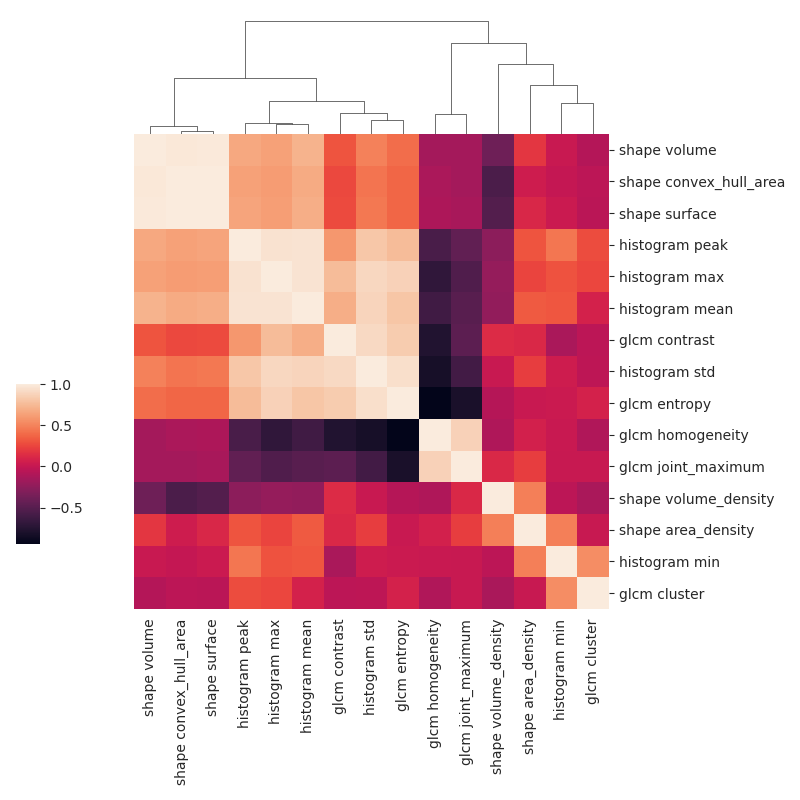
\includegraphics[width=1\textwidth]{Figures/feature_correlation.png}
    \caption{Pearson Correlation between each feature calculated on the full
    dataset. }  
    \label{fig:correlation} 
\end{figure}





%%%%%%%%%%%%%%%%%%%%%%%%%%%%%%%%%%%%%%%%%%%%%
\subsection{Compare Manual VS Automatic feature reduction}
\begin{itemize}
    \item Is the Automatic selection method as expected, compared with visual
        inspection, manual feature reduction.   
\end{itemize}




%%%%%%%%%%%%%%%%%%%%%%%%%%%%%%%%%%%%%%%%%%%%
\subsection{SVM}

\subsubsection{Classification of class 1 vs class 4}

\begin{figure}[H]
\centering
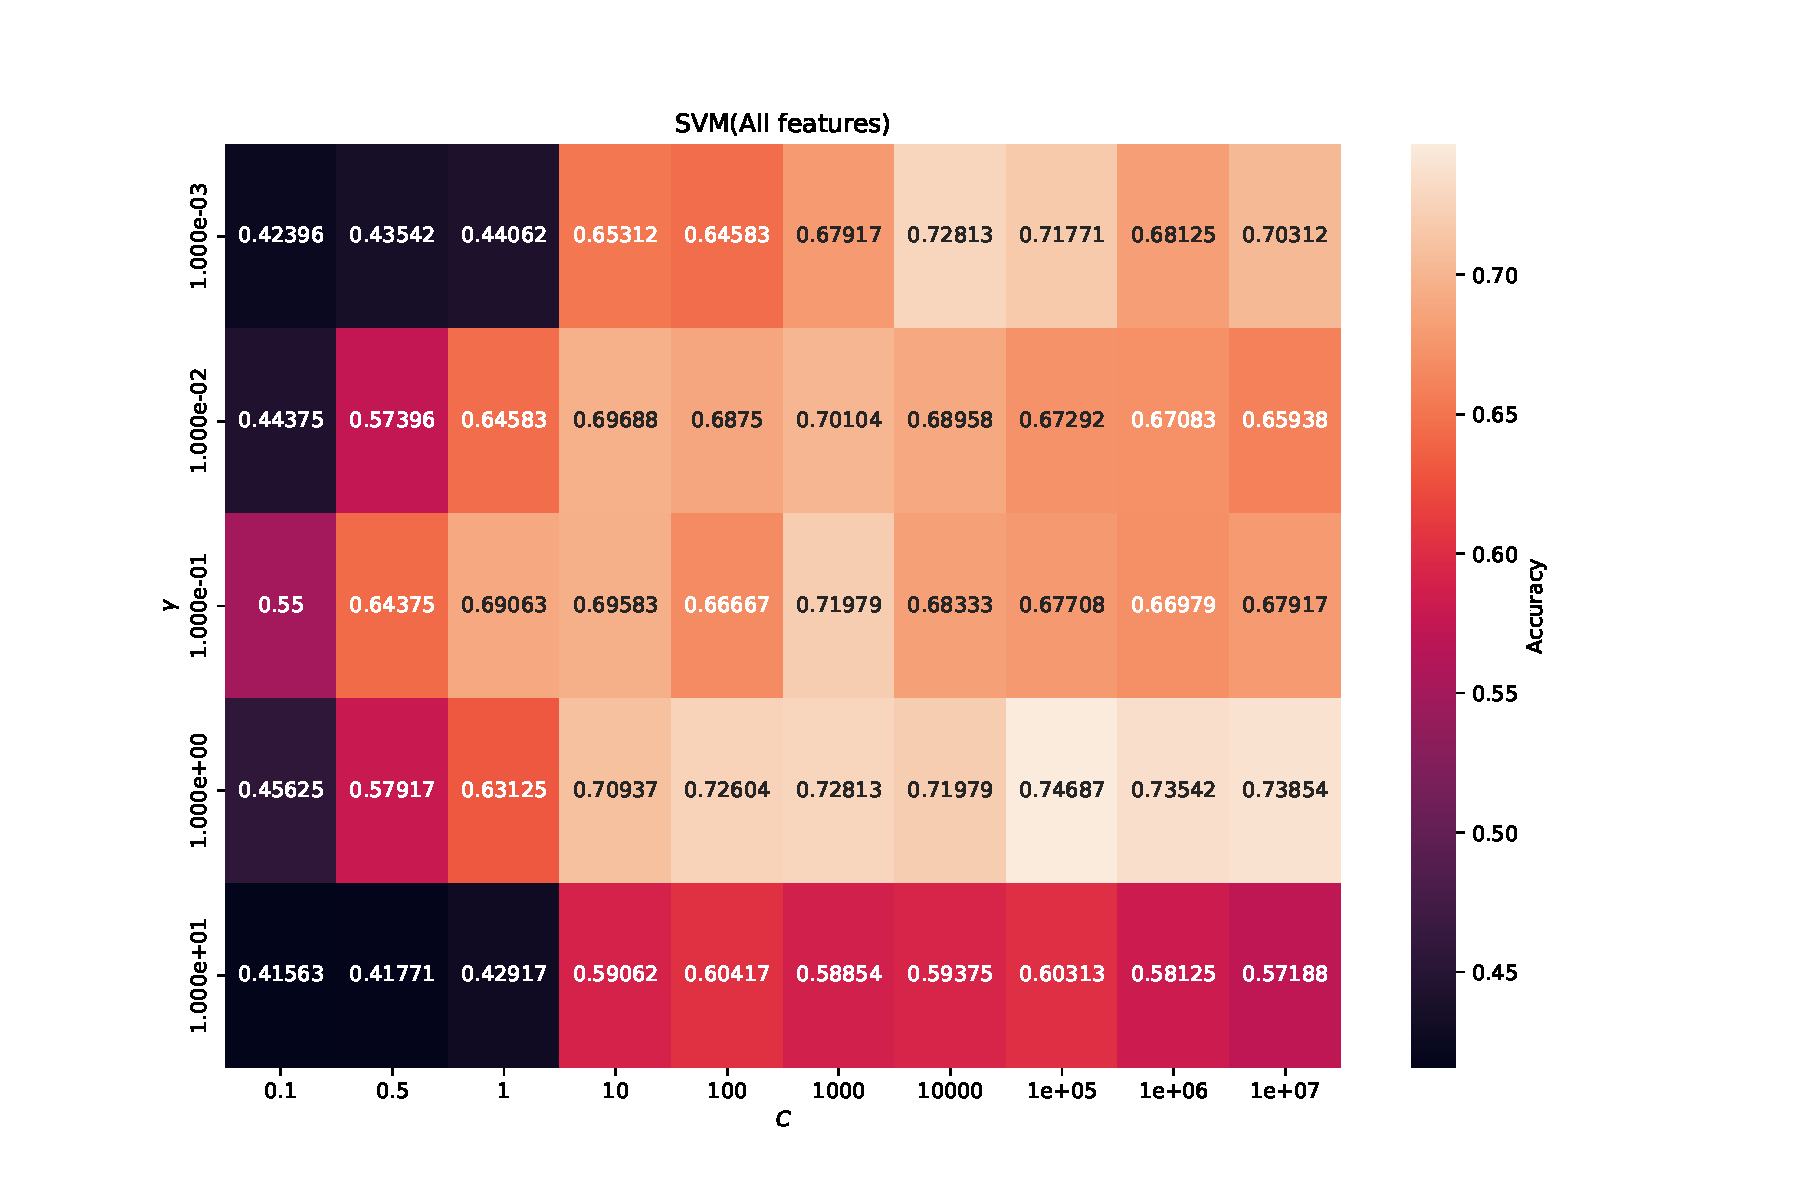
\includegraphics[width=1\textwidth]{Figures/accuracy(C,gamma)0}
\caption{Heatmap of the accuracy obtained with different slack constants $C$ and 
GRBF kernel factors $\gamma $ in the SVM model training with all the features. The SVM accuracies are the average of $30$ cross-validation 
cycles training and predicting test data of relative size $0.25$.}
\label{fig:Figures-accuracy-C-gamma-0}
\end{figure}
\autoref{fig:Figures-accuracy-C-gamma-0} shows the accuracy of the SVM model's 
test data predictions for different slack constants $C$ and GRBF kernel factors $\gamma $. 
We observe the best accuracy $0.747$ for $C=10^5$ and $\gamma =1$. Lower slack constant 
allows for more misclassification while lower $\gamma $ results in a wider 
GRBF kernel which means that the influence of each data point on the hyperplane 
position will decrease. Both leads towards under fitting on the under-over fit spectrum.
Our optimal values for $C$ and $\gamma $ are quite large suggesting the need for 
a complex hyperplane to classify our data. 

We will utilize these optimal value in our analysis of predictions based on two and three 
features. They should be tuned for every feature combination, but this would required 
way to much computation to handle for our computer. The optimal parameter values 
obtained using all the features will be good general parameters for the following 
feature combination analysis. 

\begin{figure}[H]
\centering
\makebox[\textwidth][c]{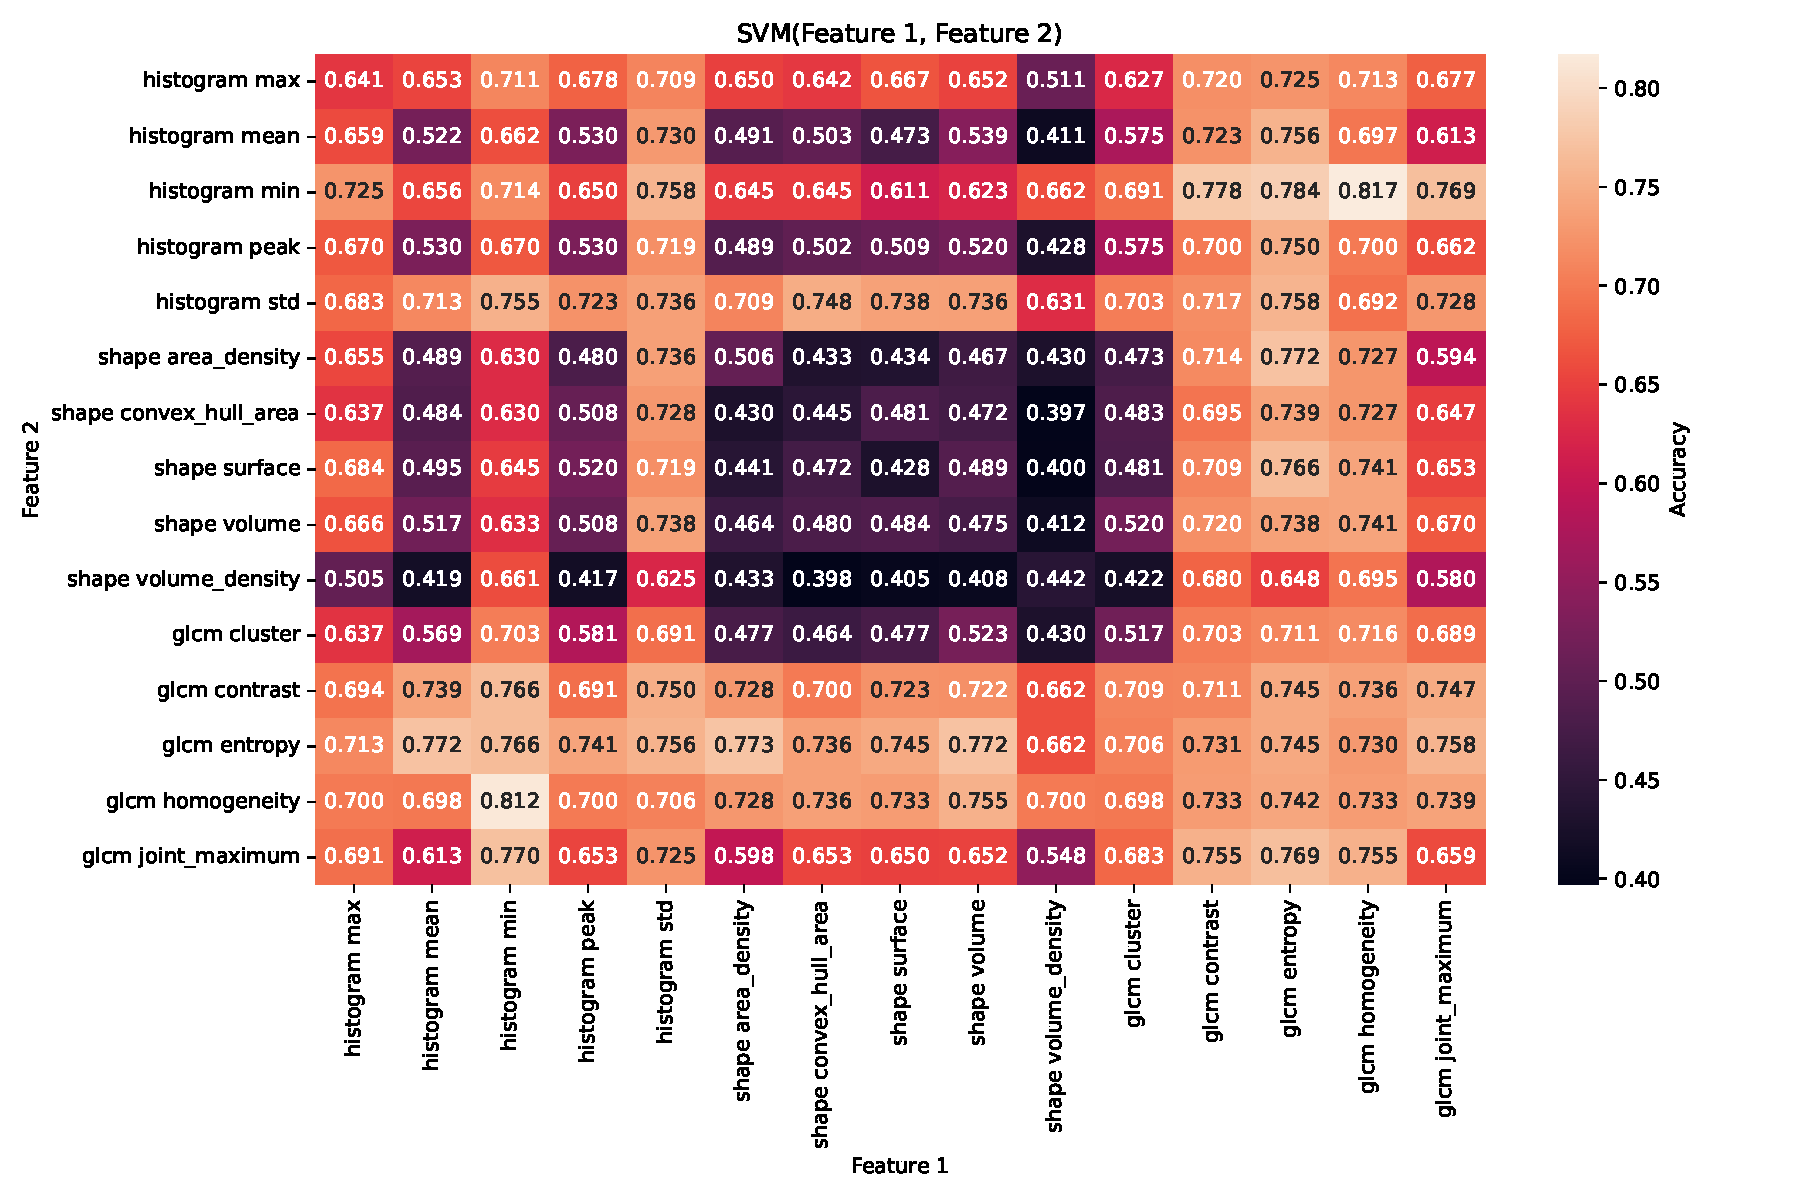
\includegraphics[width=1.2\textwidth]{Figures/feature_pairs0}}
\caption{Heatmap of the accuracy obtained by the SVM model training on different feature pairs. The SVM accuracies are the average 
of $20$ cross-validation cycles training and predicting test data of relative size $0.25$.
The slack constant and GRBF kernel factor are set to $C=10^5$  $\gamma=1 $ respectively. }
\label{fig:Figures-feature_pairs0}
\end{figure}

\autoref{fig:Figures-feature_pairs0} shows a heatmap of the accuracy obtained with different 
feature pairs utilized by the SVM model for training and predicting. The diagonal from upper left 
to lower right of the heatmap shows pairs of same features which is equivalent to classification 
based on that single feature. We observe the best score for a single feature with \verb|glcm entropy|
with accuracy $0.745$.

The accuracy of each feature pairs have been derived twice, one on either side of the equal feature diagonal, which is nice as 
this gives some conformation. We observe both scores of the feature pair \verb|histogram min| and \verb|glcm homogeneity| 
to be the best with accuracy $0.812$ and $0.817$. This feature pair is one of the combinations 
expected to give good results in \autoref{tab:expectation}. The table also shows an expected 
good result with the feature pair \verb|glcm entropy| and \verb|glcm homogeneity|, although 
our SVM analysis shows worse accuracy when including \verb|glcm homogeneity| compared to \verb|glcm entropy| 
alone. Assuming these features have low correlation as shown in \autoref{fig:correlation}, one would expect 
an increase in accuracy as both shows good accuracy on their own. Therefore the poor accuracy 
might be a result of bad parameters ($C$ and $\gamma $) for this combination of feature. The rest of the 
feature pair combinations in the rows of \autoref{tab:expectation} seem to improve the accuracy. 

\begin{figure}[H]
\centering
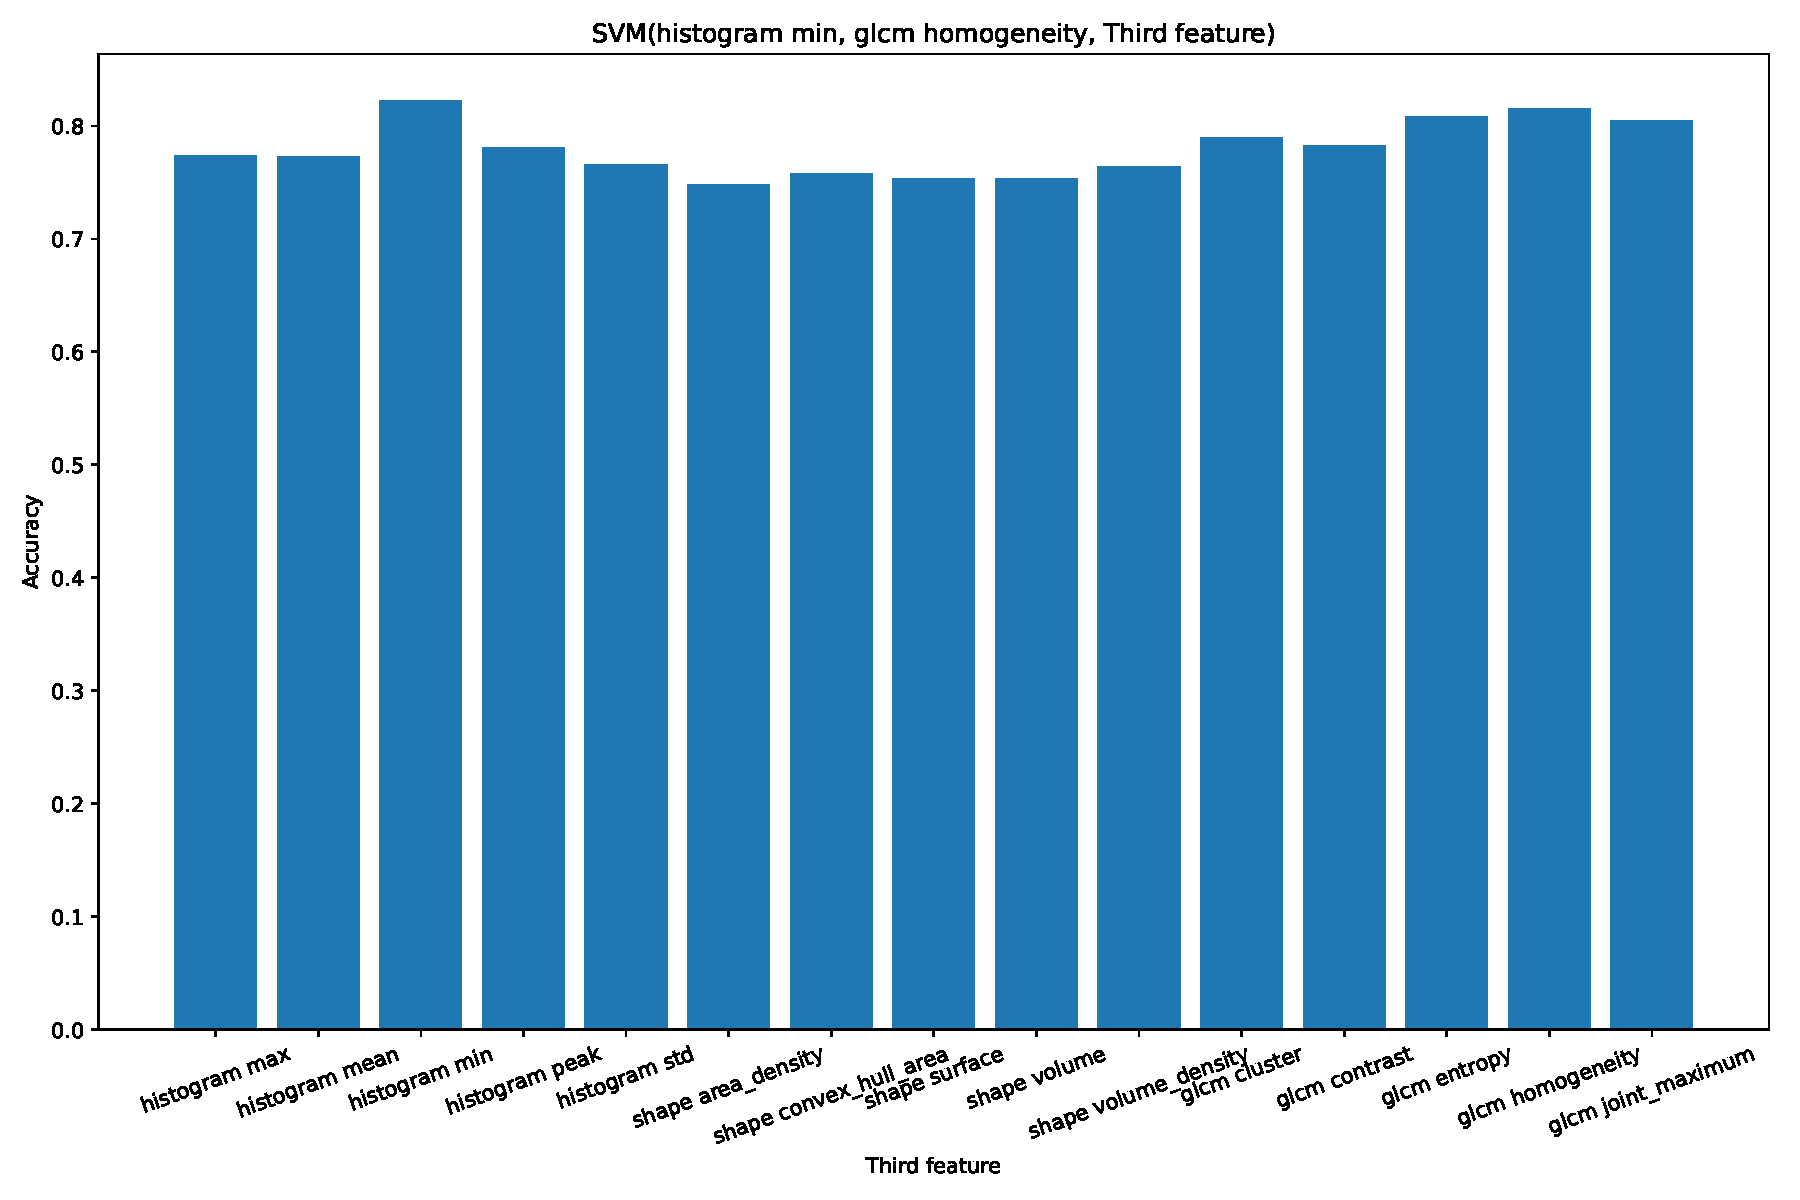
\includegraphics[width=1\textwidth]{Figures/third_feature0}
\caption{Bar plot of the accuracy obtained adding a third feature in the data used 
by the SVM model. The accuracies are the average 
of $50$ cross-validation cycles training and predicting test data of relative size $0.25$.
The slack constant and GRBF kernel factor are set to $C=10^5$  $\gamma=1 $ respectively. }
\label{fig:Figures-third_feature0}
\end{figure}

\autoref{fig:Figures-third_feature0} shows the accuracy gotten when adding a third feature to the best scoring feature pair 
\verb|histogram min| and \verb|glcm homogeneity| from \autoref{fig:Figures-feature_pairs0}. We observe best scores for 
third feature \verb|histogram min| and \verb|glcm homogeneity| which corresponds to no third feature. Thus, the addition of 
a third feature results in worse accuracy. The optimal feature pair in got better accuracy than 
what was obtained using all the features in \autoref{fig:Figures-accuracy-C-gamma-0} for which the parameters was tuned.
This suggest that there will be a point where adding more feature will decrease the prediction power of our model. 
Our results suggesting this point is for our two features should again be confirmed tuning the parameters $C$ and $\gamma $ 
for each feature combination. 
\subsubsection{Classification of class 0 vs class 4}

\begin{figure}[H]
\centering
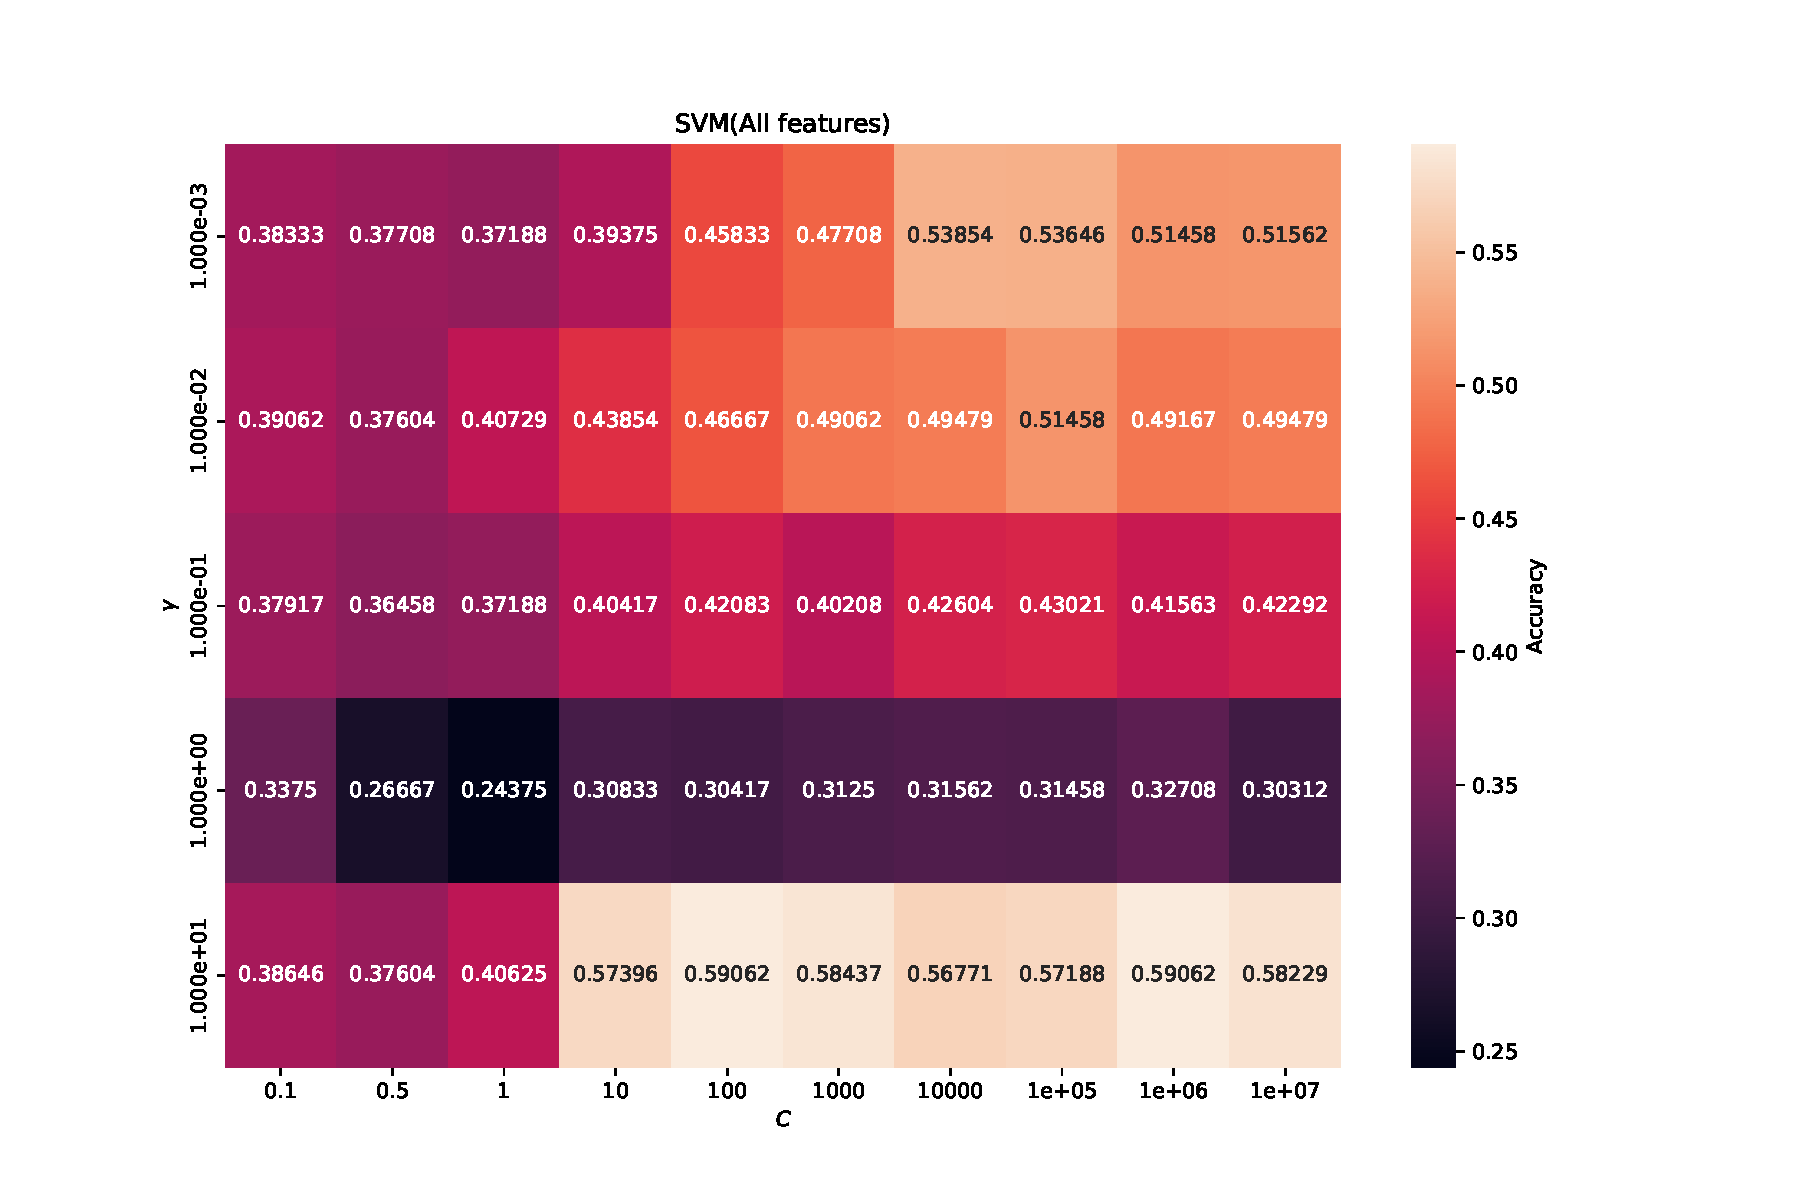
\includegraphics[width=1\textwidth]{Figures/accuracy(C,gamma)1}
\caption{Heatmap of the accuracy obtained with different slack constants $C$ and 
GRBF kernel factors $\gamma $ in the SVM model training with all the features. The SVM accuracies are the average of $30$ cross-validation 
cycles training and predicting test data of relative size $0.25$.}
\label{fig:Figures-accuracy-C-gamma-1}
\end{figure}

\begin{figure}[H]
\centering
\makebox[\textwidth][c]{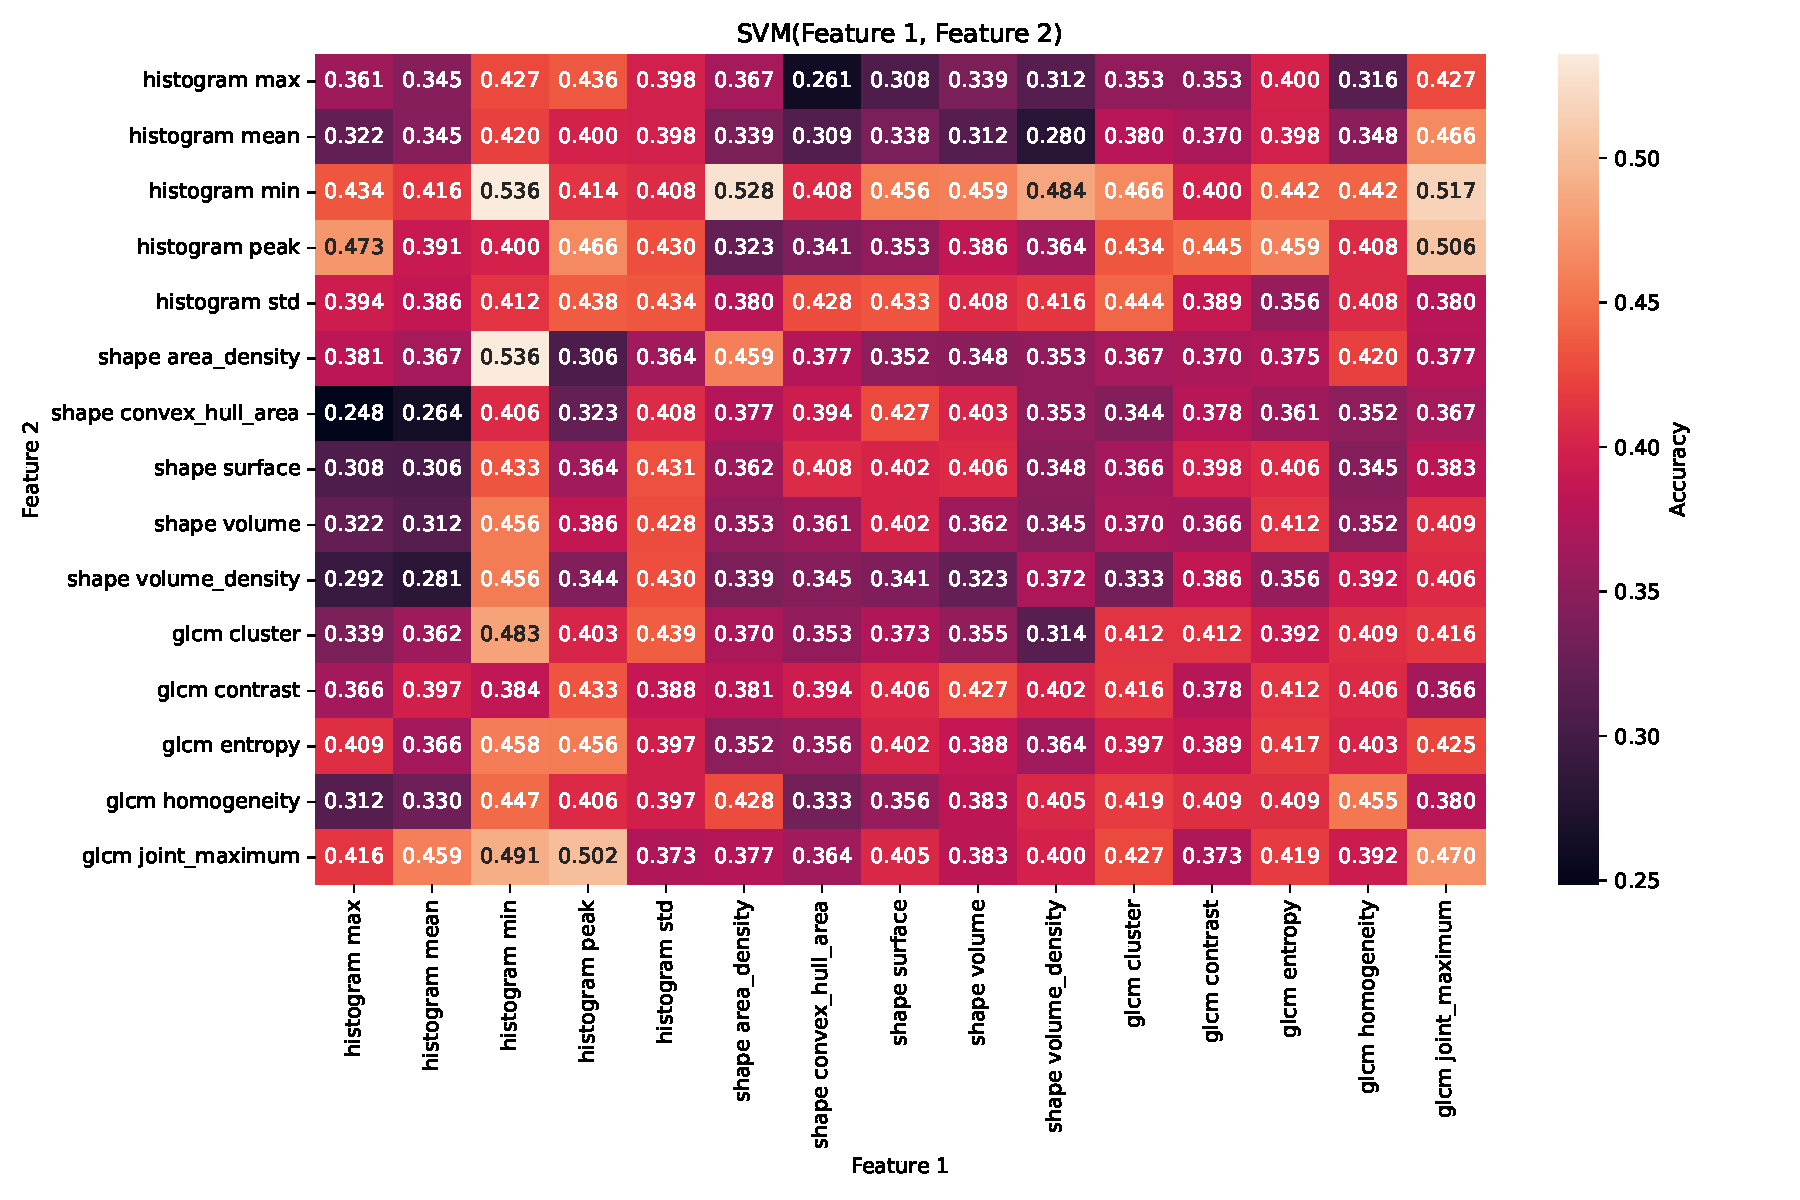
\includegraphics[width=1.2\textwidth]{Figures/feature_pairs1}}
\caption{Heatmap of the accuracy obtained by the SVM model training on different feature pairs. The SVM accuracies are the average 
of $20$ cross-validation cycles training and predicting test data of relative size $0.25$.
The slack constant and GRBF kernel factor are set to $C=100$  $\gamma=10 $ respectively. }
\label{fig:Figures-feature_pairs1}
\end{figure}

\begin{figure}[H]
\centering
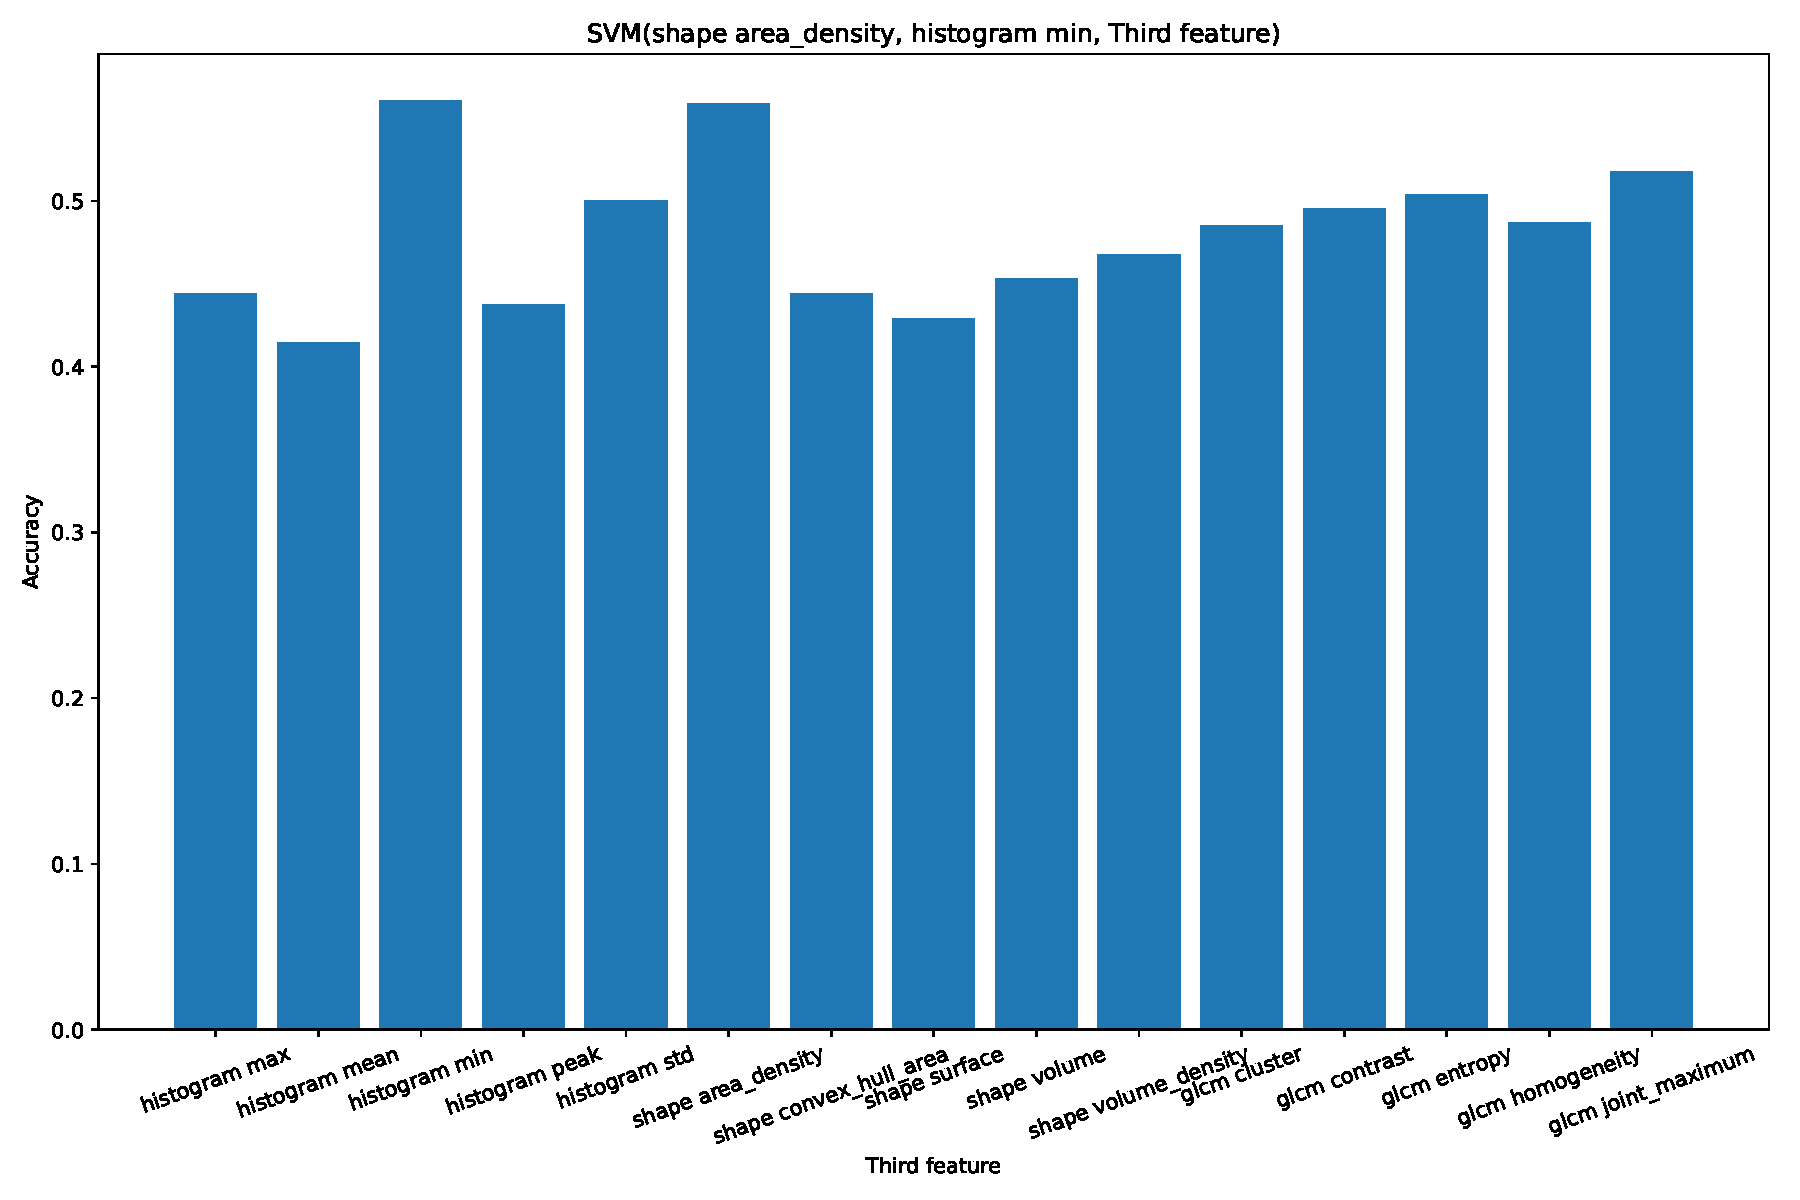
\includegraphics[width=1\textwidth]{Figures/third_feature1}
\caption{Bar plot of the accuracy obtained adding a third feature in the data used 
by the SVM model. The accuracies are the average 
of $50$ cross-validation cycles training and predicting test data of relative size $0.25$.
The slack constant and GRBF kernel factor are set to $C=100$  $\gamma=10 $ respectively. }
\label{fig:Figures-third_feature1}
\end{figure}


\subsubsection{Classification of class 0 vs class 1}

\begin{figure}[H]
\centering
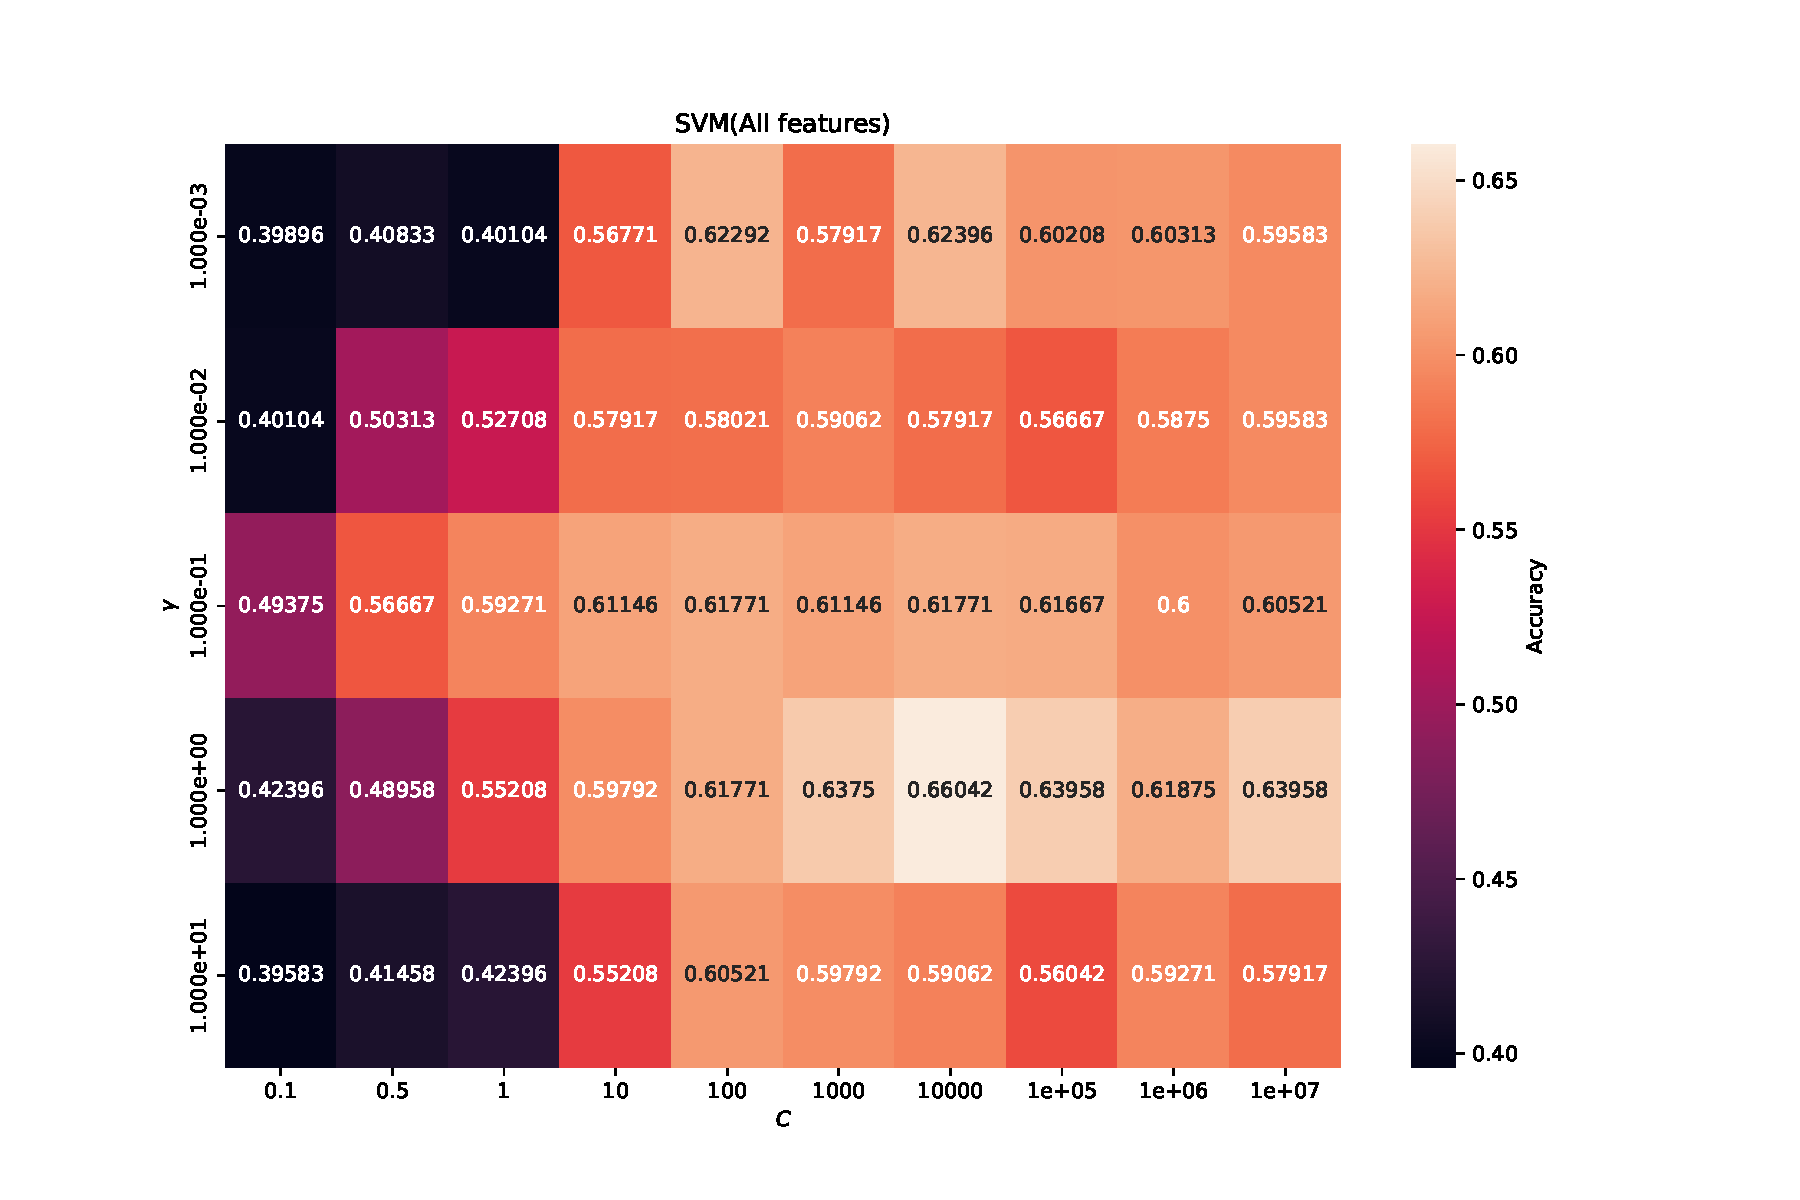
\includegraphics[width=1\textwidth]{Figures/accuracy(C,gamma)4}
\caption{Heatmap of the accuracy obtained with different slack constants $C$ and 
GRBF kernel factors $\gamma $ in the SVM model training with all the features. The SVM accuracies are the average of $30$ cross-validation 
cycles training and predicting test data of relative size $0.25$.}
\label{fig:Figures-accuracy-C-gamma-4}
\end{figure}

\begin{figure}[H]
\centering
\makebox[\textwidth][c]{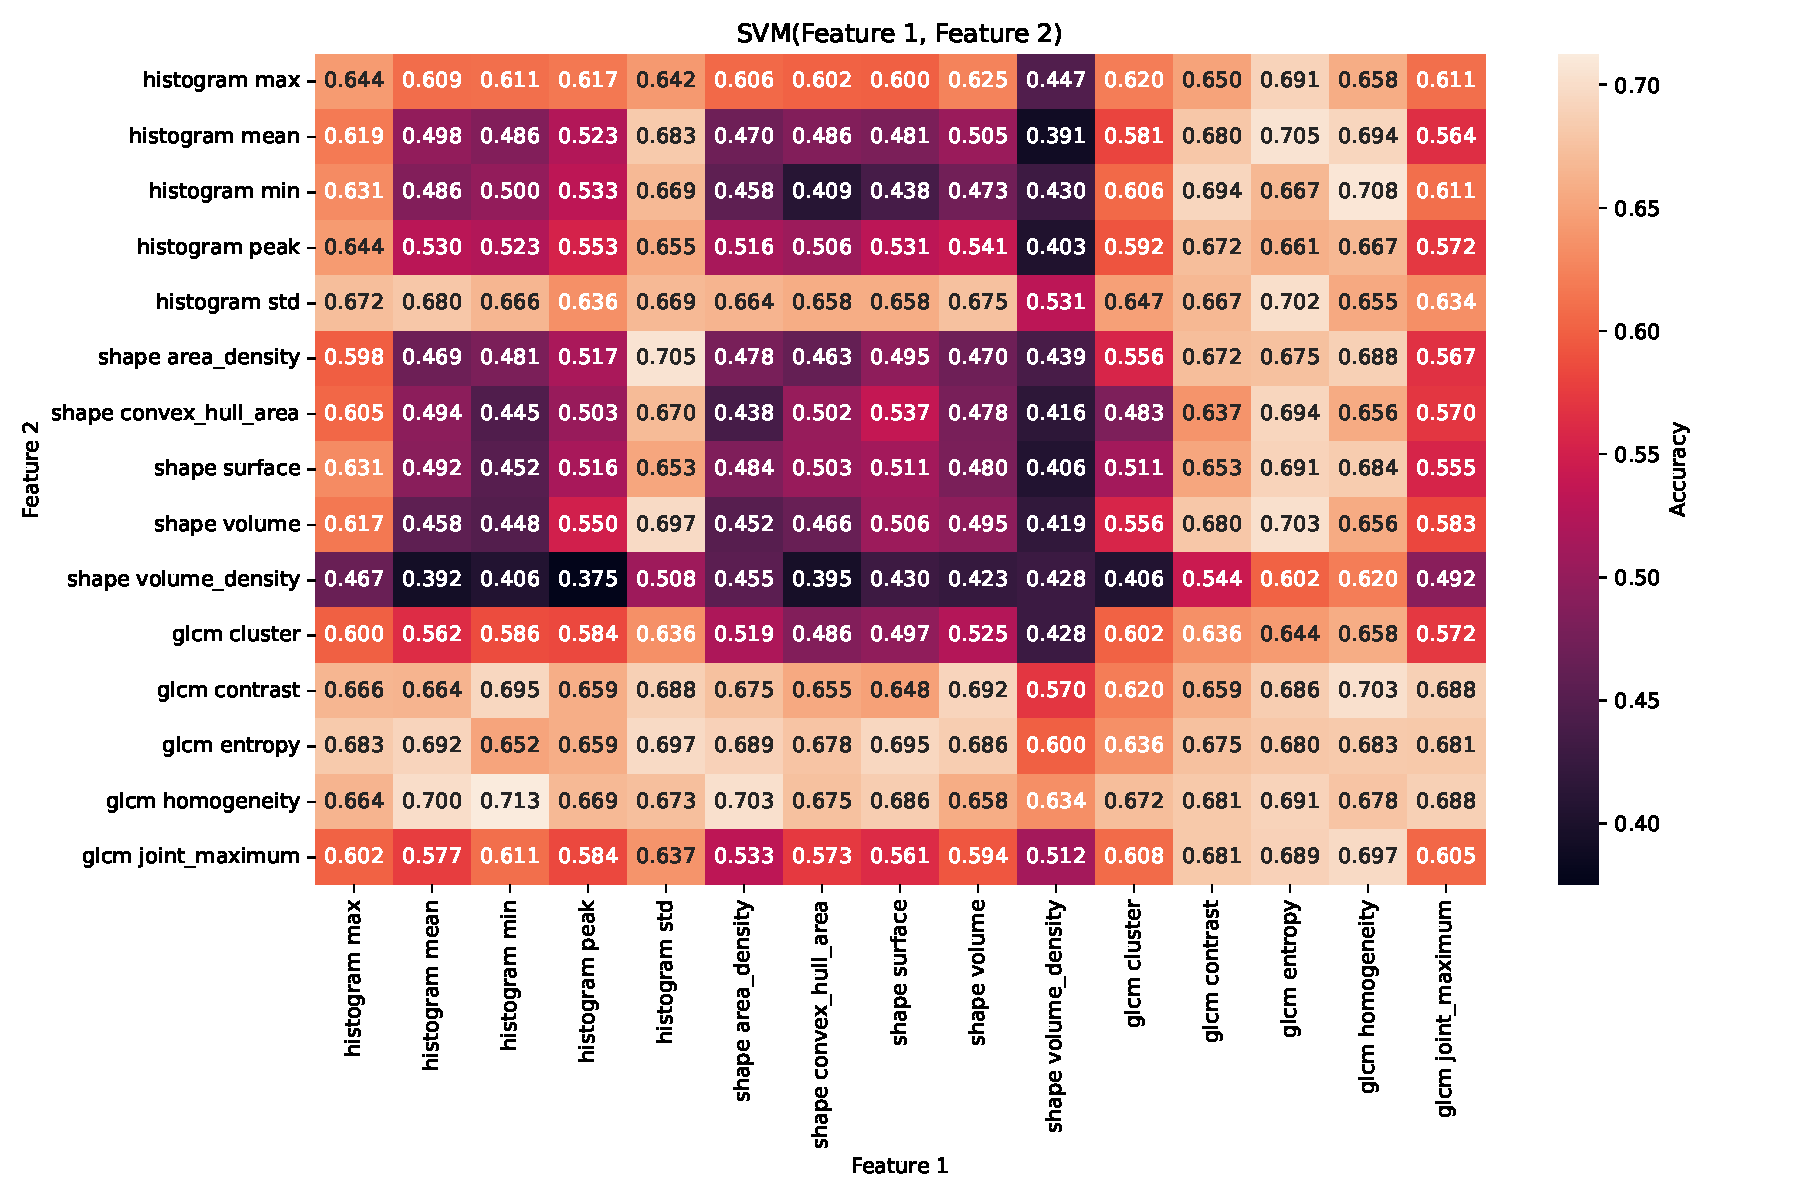
\includegraphics[width=1.2\textwidth]{Figures/feature_pairs4}}
\caption{Heatmap of the accuracy obtained by the SVM model training on different feature pairs. The SVM accuracies are the average 
of $20$ cross-validation cycles training and predicting test data of relative size $0.25$.
The slack constant and GRBF kernel factor are set to $C=10^4$  $\gamma=1 $ respectively. }
\label{fig:Figures-feature_pairs4}
\end{figure}

\begin{figure}[H]
\centering
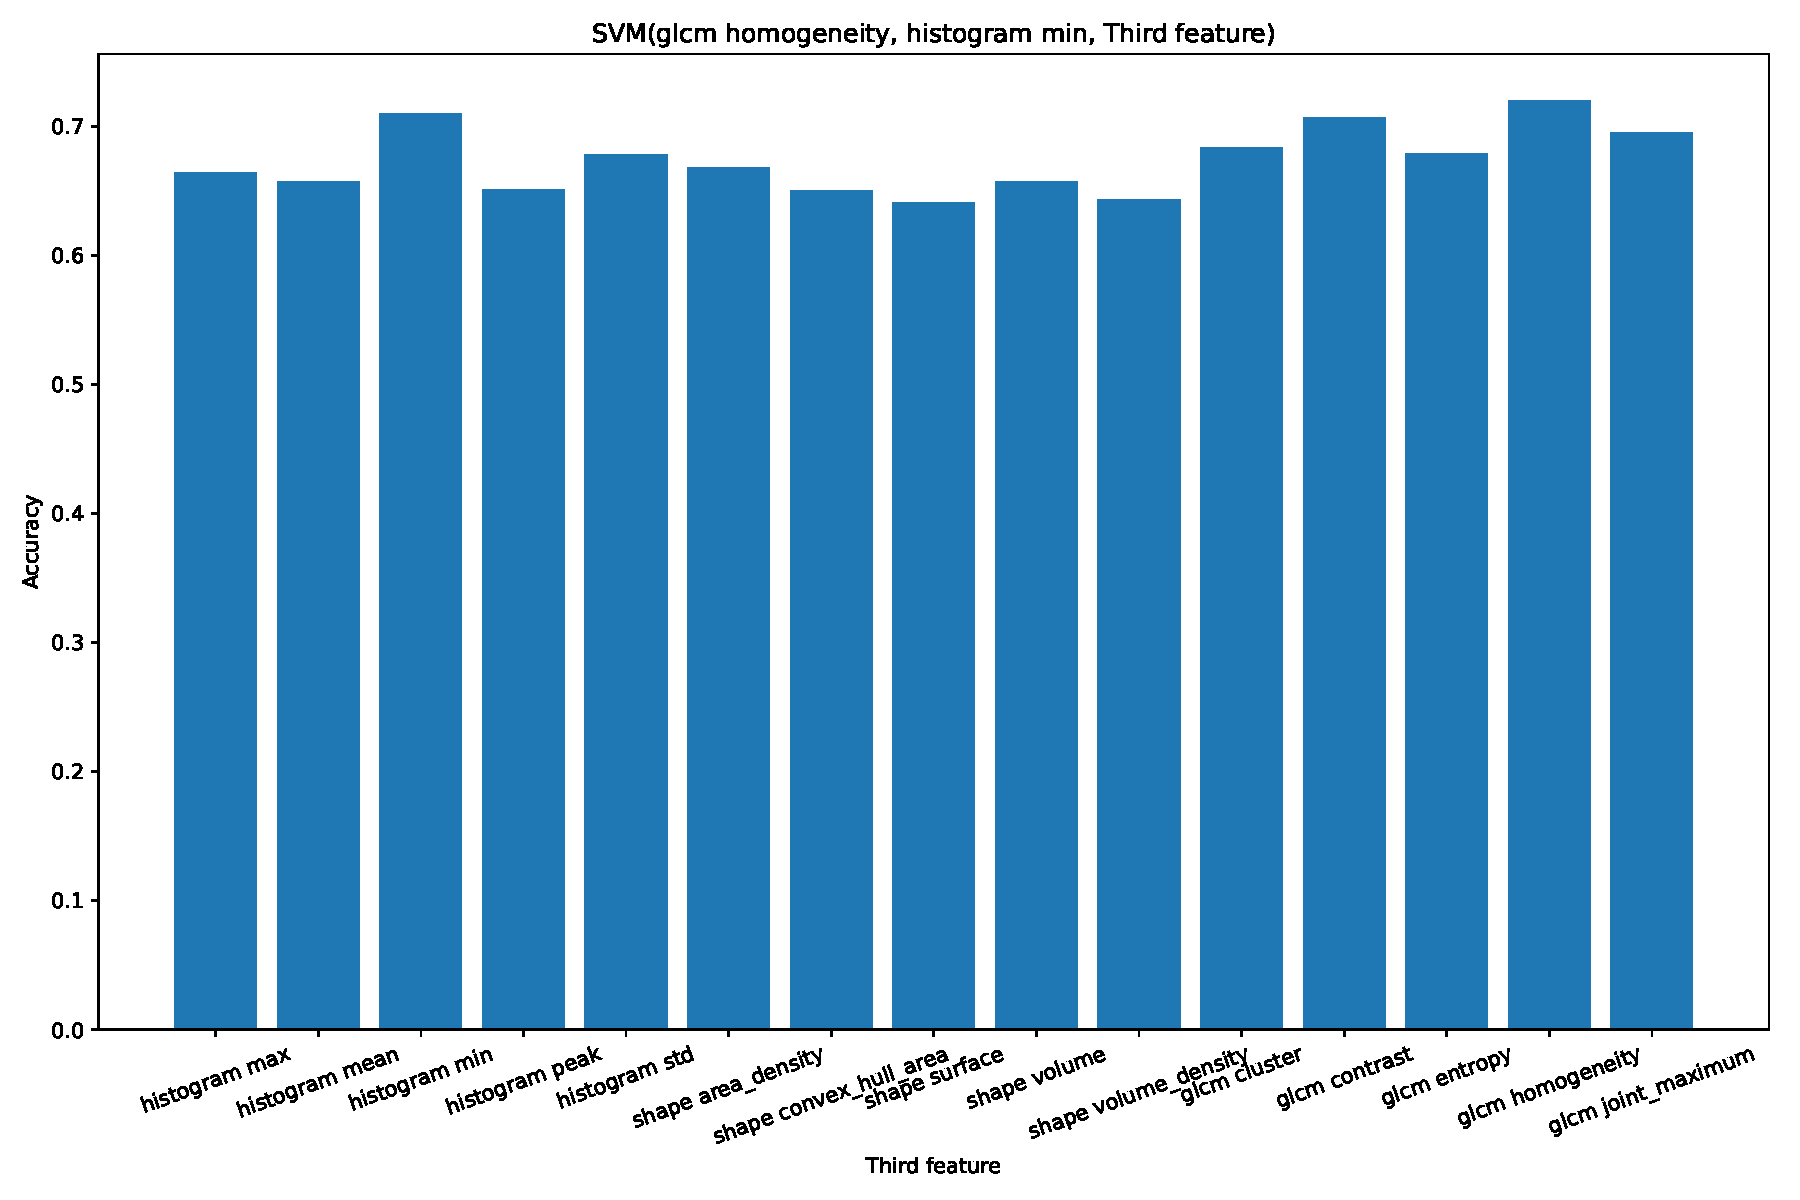
\includegraphics[width=1\textwidth]{Figures/third_feature4}
\caption{Bar plot of the accuracy obtained adding a third feature in the data used 
by the SVM model. The accuracies are the average 
of $50$ cross-validation cycles training and predicting test data of relative size $0.25$.
The slack constant and GRBF kernel factor are set to $C=10^4$  $\gamma=1 $ respectively. }
\label{fig:Figures-third_feature4}
\end{figure}








\end{document}
